% Set a pdf version and a document type
\ifx\pdfminorversion\undefined\else\pdfminorversion=4\fi
\documentclass[aspectratio=169,t,table]{beamer}

% Import all necessary packages
% Use this file to import all packages which are needed for the lecture
\usepackage[english]{babel}
\usepackage[utf8]{inputenc}
\usepackage[sfdefault]{roboto}
\usepackage[T1]{fontenc}
\usepackage{amsmath,amssymb}
\usepackage{graphicx}
\usepackage{listings}
\usepackage[backend=biber,sorting=none,doi=true,style=ieee]{biblatex}
\usepackage{url}
\usepackage{hyperref}
\usepackage{fontawesome5}
\usepackage{graphicx}
\usepackage{booktabs}
\usepackage{calc}
\usepackage{ifthen}
\usepackage{tabularx}
\usepackage{longtable}
\usepackage{makecell}
\usepackage{multicol}
\usepackage{multirow}
\usepackage{hhline}
\usepackage{qrcode}
\usepackage{xcolor}
\usepackage{cleveref}
\usepackage{tikz}
\usepackage{tikz-cd}
\usepackage{pgfplots,pgfplotstable,pgf-pie}
\usepackage[linesnumbered]{algorithm2e}
\usepackage{array}
\usepackage{mathtools}
\usetikzlibrary{patterns}
\usetikzlibrary{arrows.meta}


% Set the theme (customized FAU beamer theme)
\usetheme[%
	image,%
	longtitle,%
	inst=tf%
]{fau}

% Set all important settings and define commands that are used in more than one lecture
% English version FAU Logo
\usepackage[english]{babel}
% German version FAU Logo
%\usepackage[ngerman]{babel}

\usepackage[utf8]{inputenc}
\usepackage[T1]{fontenc}
\usepackage{amsmath,amssymb}
\usepackage{graphicx}
\usepackage{listings}
\usepackage[backend=biber,sorting=none,doi=true,style=ieee]{biblatex}

% Options:
%  - inst:      Institute
%                 med:      MedFak FAU theme
%                 nat:      NatFak FAU theme
%                 phil:     PhilFak FAU theme
%                 rw:       RWFak FAU theme
%                 rw-jura:  RWFak FB Jura FAU theme
%                 rw-wiso:  RWFak FB WISO FAU theme
%                 tf:       TechFak FAU theme
%  - image:     Cover image on title page
%  - plain:     Plain title page
%  - longtitle: Title page layout for long title
\usetheme[%
	image,%
	longtitle,%
	inst=tf%
]{fau}

% Enable semi-transparent animation preview
\setbeamercovered{transparent}

% Enable frame numbering
%\setbeamertemplate{footline}[frame number]


\lstset{%
	language=Python,
	tabsize=2,
	basicstyle=\tt,
	keywordstyle=\color{blue},
	commentstyle=\color{green!50!black},
	stringstyle=\color{red},
	numbers=left,
	numbersep=0.5em,
	xleftmargin=1em,
	numberstyle=\tt
}

\defbibheading{bibliography}{}
\addbibresource{references.bib}

\date[SS2022]{Summer semester 2022}


\usepackage{url}
\usepackage{enumitem}
\setlist[itemize]{noitemsep, nolistsep}
\setlist[itemize]{label=\footnotesize\raisebox{.275ex}{$\bullet$}}
\usepackage{hyperref}
\usepackage{fontawesome5}
\usepackage{graphicx}
\usepackage{booktabs}
\usepackage{calc}
\usepackage{ifthen}

\usepackage{tabularx}
\usepackage{makecell}

\usepackage{xcolor}
\definecolor{airforceblue}{rgb}{0.36, 0.54, 0.66}
\definecolor{ForestGreen}{rgb}{0.34, 0.139, 0.34}

% English version
\institute[CS6]{Chair of Computer Science 6 (Data Management), Friedrich-Alexander University Erlangen-N\"urnberg}
% German version
% \institute[Lehrstuhl]{Lehrstuhl, Friedrich-Alexander-Universit\"at Erlangen-N\"urnberg}

\setbeamertemplate{section in toc}[sections numbered]

\setbeamertemplate{section page}{%
	\begingroup
	\begin{beamercolorbox}[sep=10pt,center,rounded=true,shadow=true]{section title}
		\usebeamerfont{section title}\thesection~\insertsection\par
	\end{beamercolorbox}
	\endgroup
}

\usepackage{tikz}
\usepackage{tikz-cd}
\usepackage{pgfplots,pgfplotstable,pgf-pie}

\newcommand{\tikzmark}[1]{\tikz[remember picture] \node[coordinate] (#1) {#1};}

\tikzset{
	every overlay node/.style={
			%draw=black,fill=white,rounded corners,
			anchor=north west, inner sep=0pt,
		},
}
% Usage:
% \tikzoverlay at (-1cm,-5cm) {content};
% or
% \tikzoverlay[text width=5cm] at (-1cm,-5cm) {content};
\def\tikzoverlay{%
	\tikz[remember picture, overlay]\node[every overlay node]
}%

\newcommand{\plots}{0.611201}
\newcommand{\plotm}{2.19882}

\newcommand{\MaxNumberX}{3}
\newcommand{\MaxNumberY}{5}

\pgfmathdeclarefunction{gauss}{2}{%
	\pgfmathparse{1/(#2*sqrt(2*pi))*exp(-((x-#1)^2)/(2*#2^2))}%
}

\tikzset{
	thick,
	>=latex,
	every edge/.style={draw=gray, thick, >=latex},
	vertex/.style = {
			circle,
			fill            = black,
			outer sep = 2pt,
			inner sep = 1pt,
		}
}
\usetikzlibrary{matrix,mindmap}
\usetikzlibrary{arrows,decorations.pathmorphing,backgrounds,fit,positioning,shapes.symbols,chains,intersections,snakes}
\tikzset{level 1/.append style={sibling angle=50,level distance = 165mm}}
\tikzset{level 2/.append style={sibling angle=20,level distance = 45mm}}
\tikzset{every node/.append style={scale=1}}
% read in data file
\pgfplotstableread{data/iris.dat}\iris
% get number of data points
\pgfplotstablegetrowsof{\iris}
\pgfmathsetmacro\NumRows{\pgfplotsretval-1}

\usepgfplotslibrary{groupplots}
\pgfplotsset{height=4cm,width=8cm,compat=1.14}

\tikzset{
	vertex/.style = {
			circle,
			fill            = black,
			outer sep = 2pt,
			inner sep = 1pt,
		}
}

\tikzset{
	mynode/.style={
			draw,
			thick,
			anchor=south west,
			minimum width=2cm,
			minimum height=1.3cm,
			align=center,
			inner sep=0.2cm,
			outer sep=0,
			rectangle split,
			rectangle split parts=2,
			rectangle split draw splits=false},
	reverseclip/.style={
			insert path={(current page.north east) --
					(current page.south east) --
					(current page.south west) --
					(current page.north west) --
					(current page.north east)}
		}
}

\tikzset{basic/.style={
			draw,
			rectangle split,
			rectangle split parts=2,
			rectangle split part fill={blue!20,white},
			minimum width=2.5cm,
			text width=2cm,
			align=left,
			font=\itshape
		},
	Diamond/.style={ diamond,
			draw,
			shape aspect=2,
			inner sep = 2pt,
			text centered,
			fill=blue!10!white,
			font=\itshape
		}}


\tikzset{level 1/.append style={sibling angle=50,level distance = 165mm}}
\tikzset{level 2/.append style={sibling angle=20,level distance = 45mm}}
\tikzset{every node/.append style={scale=1}}

\usetikzlibrary{arrows,decorations.pathmorphing,backgrounds,fit,positioning,shapes.symbols,chains,intersections,snakes,positioning,matrix,mindmap,shapes.multipart,shapes,calc,shapes.geometric}



% Title, author(s), and date
\title[KDD~7.~Classification]{7. Classification} %
\subtitle{Knowledge Discovery in Databases}
\author[D.~Probst]{Dominik Probst, \texttt{dominik.probst@fau.de}}

\input{x-additional/vc.tex}

\hypersetup{
	pdfkeywords={},
	pdfsubject={Version \GITAbrHash},
	pdfcreator={},
	pdflang={English}
}


% Create custom commands
\newcommand\mycommfont[1]{\footnotesize\ttfamily\textcolor{faucyan}{#1}}
\newcommand*\revealcline{\noalign{\vskip\arrayrulewidth}} % used in 5-evaluation-selection

% Set custom (theme) settings 
\setbeamercovered{invisible}
\SetCommentSty{mycommfont}

% Start the document
\begin{document}

% Title
\maketitle

{ % Outline
	\setbeamertemplate{footline}{}
	\begin{frame}[noframenumbering]{Outline}
		\tableofcontents

	\end{frame}
}

% Body
\section{Basic Concepts}

\begin{frame}{What is Frequent-pattern Analysis?}
	\begin{itemize}
		\item \textbf{Frequent pattern:}
		      \begin{itemize}
			      \item A pattern (a set of items, subsequences, substructures, etc.)
			            that occurs frequently in a dataset.
		      \end{itemize}
		\item \textbf{Motivation: Finding inherent regularities in data:}
		      \begin{itemize}
			      \item What products are often purchased together? Beer and diapers?!
			      \item What are the subsequent purchases after buying a PC?
			      \item Who bought this has often also bought $\ldots$"
			      \item What kinds of DNA are sensitive to this new drug?
			      \item Can we automatically classify Web documents?
		      \end{itemize}
		\item \textbf{Applications:}
		      \begin{itemize}
			      \item Basket-data analysis, cross-marketing, catalog design,
			            sale-campaign analysis, Web-log (click-stream) analysis, and
			            DNA-sequence analysis.
		      \end{itemize}
	\end{itemize}
\end{frame}

\begin{frame}{Why is Frequent-pattern Mining Important?}
	\begin{itemize}
		\item \textbf{A frequent pattern is an intrinsic and important property
			      of a dataset.}
		\item \textbf{Foundation for many essential data-mining tasks:}
		      \begin{itemize}
			      \item Association, correlation, and causality analysis.
			      \item Sequential, structural (e.g., sub-graph) patterns.
			      \item Pattern analysis in spatiotemporal, multimedia, time-series,
			            and stream data.
			      \item Classification: discriminative, frequent-pattern analysis.
			      \item Cluster analysis: frequent-pattern-based clustering.
			      \item Data warehousing: iceberg cube and cube gradient.
			      \item Semantic data compression: fascicles (Jagadish, Madar, and
			            Ng, VLDB'99).
			      \item Broad applications.
		      \end{itemize}
	\end{itemize}
\end{frame}

\begin{frame}{An Example}
	\begin{itemize}
		\item \textbf{From: Martin Lindstrom: Brandwashed. Random House, 2011:}
		      \begin{quote}
			      It is by crunching these numbers that the data-mining industry has
			      uncovered some even more surprising factoids:

			      Did you know, for example, that at Walmart a shopper who buys a
			      Barbie doll is 60 percent more likely to purchase one of three
			      types of candy bars? Or that toothpaste is most often bought
			      alongside canned tuna? Or that a customer who buys a lot of meat is
			      likely to spend more money in a health-food store than a
			      non-meat-eater? Or what about the data revealed to one Canadian
			      grocery chain that customers who bought coconuts also tended to buy
			      prepaid calling cards? At first, no one in store management could
			      figure out what was going on. What could coconuts possibly have to
			      do with calling cards?

			      Finally it occurred to them that the store served a huge population
			      of shoppers from the Caribbean islands and Asia, both of whose
			      cuisines use coconuts in their cooking. Now it made perfect sense
			      that these Caribbean and Asian shoppers were buying prepaid calling
			      cards to check in with their extended families back home.
		      \end{quote}
	\end{itemize}
\end{frame}

\begin{frame}{An Example}
	\begin{columns}
		\begin{column}{0.4\textwidth}
			\begin{tabular}{|c|c|}
				\hline
				\textbf{TID} & \textbf{Items bought}             \\\hline
				10           & Beer, Nuts, Diapers               \\\hline
				20           & Beer, Coffee, Diapers             \\\hline
				30           & Beer, Diapers, Eggs               \\\hline
				40           & Nuts, Eggs, Milk                  \\\hline
				50           & Nuts, Coffee, Diapers, Eggs, Milk \\\hline
			\end{tabular}
			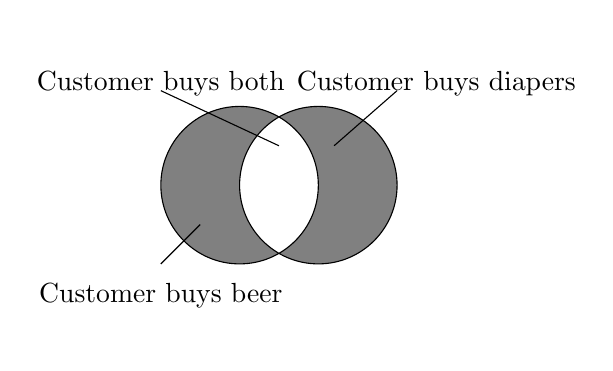
\begin{tikzpicture}[fill=gray]
				% left hand
				\scope
				\clip (-2,-2) rectangle (2,2)
				(1,0) circle (1);
				\fill (0,0) circle (1);
				\endscope
				% right hand
				\scope
				\clip (-2,-2) rectangle (2,2)
				(0,0) circle (1);
				\fill (1,0) circle (1);
				\endscope
				% outline
				\draw (0,0) circle (1) (0,1) (1,0) circle (1) (1,1);
				\node[label=below:{Customer buys beer}] at (-1,-1) {};
				\node[label=below:{Customer buys diapers}] at (2.5,1.7) {};
				\node[label=below:{Customer buys both}] at (-1,1.7) {};
				\draw (-1,-1) -- (-0.5,-0.5);
				\draw (2,1.2) -- (1.2,0.5);
				\draw (-1,1.2) -- (0.5,0.5);
			\end{tikzpicture}
		\end{column}
		\begin{column}{0.5\textwidth}
			\vspace{-2cm}
			\begin{itemize}
				\item \textbf{Itemset:}
				      \begin{itemize}
					      \item A set of one or more items.
					      \item $k$-itemset $X = \{x_1, x_2, \ldots, x_k\}$.
				      \end{itemize}
				\item \textbf{(Absolute) Support, or support count of $X$:}
				      \begin{itemize}
					      \item Frequency or occurrence of $X$.
				      \end{itemize}
				\item (Relative) Support $s$:
				      \begin{itemize}
					      \item The fraction of the transactions that contain $X$.
					      \item I.e. the \textbf{probability} that a transaction
					            contains $X$.
				      \end{itemize}
				\item \textbf{An itemset $X$ is frequent, if $X$'s support is
					      no less than a \texttt{min\_sup} threshold.}
			\end{itemize}
		\end{column}
	\end{columns}
\end{frame}

\begin{frame}{An Example}
	\begin{columns}
		\begin{column}{0.4\textwidth}
			\begin{tabular}{|c|c|}
				\hline
				\textbf{TID} & \textbf{Items bought}             \\\hline
				10           & Beer, Nuts, Diapers               \\\hline
				20           & Beer, Coffee, Diapers             \\\hline
				30           & Beer, Diapers, Eggs               \\\hline
				40           & Nuts, Eggs, Milk                  \\\hline
				50           & Nuts, Coffee, Diapers, Eggs, Milk \\\hline
			\end{tabular}
			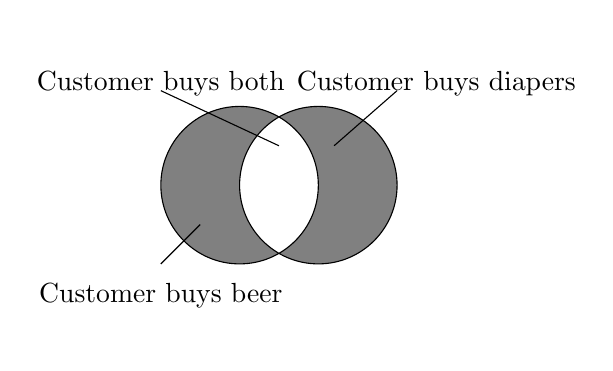
\begin{tikzpicture}[fill=gray]
				% left hand
				\scope
				\clip (-2,-2) rectangle (2,2)
				(1,0) circle (1);
				\fill (0,0) circle (1);
				\endscope
				% right hand
				\scope
				\clip (-2,-2) rectangle (2,2)
				(0,0) circle (1);
				\fill (1,0) circle (1);
				\endscope
				% outline
				\draw (0,0) circle (1) (0,1) (1,0) circle (1) (1,1);
				\node[label=below:{Customer buys beer}] at (-1,-1) {};
				\node[label=below:{Customer buys diapers}] at (2.5,1.7) {};
				\node[label=below:{Customer buys both}] at (-1,1.7) {};
				\draw (-1,-1) -- (-0.5,-0.5);
				\draw (2,1.2) -- (1.2,0.5);
				\draw (-1,1.2) -- (0.5,0.5);
			\end{tikzpicture}
		\end{column}
		\begin{column}{0.5\textwidth}
			\vspace{-2cm}
			\begin{itemize}
				\item \textbf{Find all the rules $X \implies Y$ with minimum
					      support and confidence.}
				      \begin{itemize}
					      \item \textbf{Support} $s$: probability that a transaction
					            contains $X \cup Y$.
					      \item \textbf{Confidence} $c$: conditional probability that
					            a transaction having $X$ also contains $Y$.
				      \end{itemize}
				\item \textbf{Example:}
				      \begin{itemize}
					      \item $\text{min\_sup} = 50\%$ and $\text{min\_conf} =
						            50\%$.
					      \item Frequent itemsets:
					            \begin{itemize}
						            \item Beer: $3$, Nuts: $3$, Diapers: $4$, Eggs: $3$,
						                  $\{\text{Beer, Diapers}\}$: $3$.
					            \end{itemize}
					      \item \textbf{Association rules:}
					            \begin{itemize}
						            \item Beer $\implies$ Diapers ($60\%$, $100\%$).
						            \item Diapers $\implies$ Beer ($60\%$, $75\%$).
					            \end{itemize}
				      \end{itemize}
			\end{itemize}
		\end{column}
	\end{columns}
\end{frame}

\begin{frame}{Basic Concepts: Association Rules (2)}
	\begin{itemize}
		\item \textbf{Implication of the form $A \implies B$:}
		      \begin{itemize}
			      \item where $A \neq \emptyset$, $B \neq \emptyset$ and $A \cap B =
				            \emptyset$.
		      \end{itemize}
		\item \textbf{Strong rule:}
		      \begin{itemize}
			      \item Satisfies both $\text{min\_sup}$ and $\text{min\_conf}$
			            \begin{align*}
				            \text{support}(A \implies B)    & = P(A \cup B),                                        \\
				            \text{confidence}(A \implies B) & = P(B | A)                                            \\
				                                            & = \frac{\text{support}(A \cup B)}{\text{support}(A)}.
			            \end{align*}
			      \item I.e. confidence of rule can be easily derived from the
			            support counts of $A$ and $A \cup B$.
		      \end{itemize}
		\item \textbf{Association-rule mining:}
		      \begin{itemize}
			      \item Find all frequent itemsets.
			      \item Generate strong association rules from the frequent itemsets.
		      \end{itemize}
	\end{itemize}
\end{frame}

\begin{frame}{Closed Itemsets and Max-itemsets}
	\begin{itemize}
		\item \textbf{A long itemset contains a combinatorial number of
			      sub-itemsets.}
		      \begin{itemize}
			      \item E.g. $\{a_1,a_2,\ldots,a_{100}\}$ contains
			            \begin{align*}
				            {100\choose 1} + {100 \choose 2} + \cdots + {100 \choose 100} =
				            2^{100}-1 \approx 1.27 \cdot 10^{30} \; \text{sub-itemsets!}
			            \end{align*}
			      \item \textbf{Solution:}
			            \begin{itemize}
				            \item Mine closed itemsets and max-itemsets instead.
			            \end{itemize}
			      \item \textbf{An itemset $X$ is closed, if $X$ is frequent and
				            there exists no super-itemset $X \subset Y$ with the same support
				            as $X$.} (Pasquier et al., ICDT'99)
			      \item \textbf{An itemset $X$ is a max-itemset, if $X$ is frequent
				            and there exists no frequent super-itemset $X \subset Y$.}
			            (Bayardo, SIGMOD'98)
			      \item \textbf{Closed itemset is a lossless "compression" of
				            frequent itemsets.}
			            \begin{itemize}
				            \item Reducing the number of itemsets (and rules).
			            \end{itemize}
		      \end{itemize}
	\end{itemize}
\end{frame}

\begin{frame}{Closed Itemsets and Max-itemsets (II)}
	\begin{itemize}
		\item \textbf{Example:}
		      \begin{itemize}
			      \item $\text{DB} = \{\langle a_1,a_2, \ldots, a_{100} \rangle,
				            \langle a_1, a_2, \ldots, a_{50} \rangle \}$.
			      \item I.e. just two transactions.
			      \item $\text{min\_sup} = 1$.
		      \end{itemize}
		\item \textbf{What are the closed itemsets?}
		      \begin{itemize}
			      \item $\langle a_1,a_2, \ldots, a_{100} \rangle : 1$,
			      \item $\langle a_1,a_2, \ldots, a_{50} \rangle : 2$,
			      \item Number behind the colon: support\_count.
		      \end{itemize}
		\item \textbf{What are the max-itemsets?}
		      \begin{itemize}
			      \item $\langle a_1,a_2, \ldots, a_{100} \rangle : 1$.
		      \end{itemize}
		\item \textbf{What is the set of all frequent itemsets?}
	\end{itemize}
\end{frame}

\section{Decision Tree Induction}

\begin{frame}{Decision Tree: An Example}
	\begin{columns}
		\begin{column}{0.38\textwidth}
			\vspace{-3cm}
			\begin{itemize}
				\item \textbf{Training dataset: buys\_computer.}\newline
				      The dataset follows an example of Quinlan's ID3.
				\item \textbf{Resulting tree:}\\[0.1cm]
			\end{itemize}
			\centering
			\begin{tikzpicture}[
		overlay,
		remember picture,
		>=latex,
		thick,
		node/.style={
				draw=faugray,
				rounded corners=.25em,
				fill=faugray!62,
				text depth=0.2em
			},
		leaf/.style={
				draw,
				rounded corners=.7em,
				text depth=0.2em
			},
		branch/.style={
				fill=white,
				font=\ttfamily\scriptsize,
				rounded corners=.7em,
				text depth=0.2em
			}
	]
	\node[node] at (0,0) (age) {age?};
	\node[leaf,text=faugreen,below=6.2em of age] (age-yes) {yes};

	\node[node,below left=2em and 1.5em of age] (student) {student?};
	\node[leaf,text=faured,below right=2.5em and -1em of student] (student-no) {no};
	\node[leaf,text=faugreen,below left=2.5em and -1em of student] (student-yes) {yes};

	\node[node,below right=2em and .6em of age] (credit-rating) {credit rating?};
	\node[leaf,text=faured,below left=2.5em and -2em of credit-rating] (credit-no) {no};
	\node[leaf,text=faugreen,below right=2.5em and -2em of credit-rating] (credit-yes) {yes};

	\draw (age.south) -- (age-yes.north);
	\node[branch,below=4em of age.north] {31\dots 40};

	\draw[rounded corners=5pt]
	(age.south) -- ($(age.south) + (0,-1em)$) --
	($(student.north) + (0,1em)$) -- (student.north);
	\node[branch,above=1em of student.north] {$\leq$30};

	\path[draw,rounded corners=5pt]
	(age.south) -- ($(age.south) + (0,-1em)$) --
	($(credit-rating.north) + (0,1em)$) -- (credit-rating.north);
	\node[branch,above=1em of credit-rating.north] {>40};

	% student labels
	\draw[rounded corners=5pt]
	(student.south) -- ($(student.south) + (0,-1.5em)$) --
	($(student-no.north) + (0,1em)$) -- (student-no.north);
	\node[branch,above=1em of student-no.north] {no};

	\draw[rounded corners=5pt]
	(student.south) -- ($(student.south) + (0,-1.5em)$) --
	($(student-yes.north) + (0,1em)$) -- (student-yes.north);
	\node[branch,above=1em of student-yes.north] {yes};

	% credit-rating labels
	\draw[rounded corners=5pt]
	(credit-rating.south) -- ($(credit-rating.south) + (0,-1.5em)$) --
	($(credit-no.north) + (0,1em)$) -- (credit-no.north);
	\node[branch,above=1em of credit-no.north] {excellent};

	\draw[rounded corners=5pt]
	(credit-rating.south) -- ($(credit-rating.south) + (0,-1.5em)$) --
	($(credit-yes.north) + (0,1em)$) -- (credit-yes.north);
	\node[branch,above=1em of credit-yes.north] {fair};
\end{tikzpicture}

		\end{column}
		\begin{column}{0.62\textwidth}
			\small
			\begin{tabular}{|l|l|c|c|c|}
	\hline
	\rowcolor{faugray!62}\textbf{age} & \textbf{income} & \textbf{student} & \textbf{credit\_rating} & \textbf{buys\_computer} \\\hline
	$\leq 30$                         & high            & no               & fair                    & {\color{faured}no}      \\\hline
	$\leq 30$                         & high            & no               & excellent               & {\color{faured}no}      \\\hline
	$31\ldots40$                      & high            & no               & fair                    & {\color{faugreen}yes}   \\\hline
	$>40$                             & medium          & no               & fair                    & {\color{faugreen}yes}   \\\hline
	$>40$                             & low             & yes              & fair                    & {\color{faugreen}yes}   \\\hline
	$>40$                             & low             & yes              & excellent               & {\color{faured}no}      \\\hline
	$31\ldots40$                      & low             & yes              & excellent               & {\color{faugreen}yes}   \\\hline
	$\leq 30$                         & medium          & no               & fair                    & {\color{faured}no}      \\\hline
	$\leq 30$                         & low             & no               & fair                    & {\color{faugreen}yes}   \\\hline
	$>40$                             & medium          & yes              & fair                    & {\color{faugreen}yes}   \\\hline
	$\leq 30$                         & medium          & yes              & excellent               & {\color{faugreen}yes}   \\\hline
	$31\ldots40$                      & medium          & no               & excellent               & {\color{faugreen}yes}   \\\hline
	$31\ldots40$                      & high            & yes              & fair                    & {\color{faugreen}yes}   \\\hline
	$>40$                             & medium          & no               & excellent               & {\color{faured}no}      \\\hline
\end{tabular}

		\end{column}
	\end{columns}
\end{frame}


\begin{frame}{Decision Tree}
	\vspace*{-0.6em}
	\begin{block}{Decision Tree Induction}
		\textit{Decision tree induction} refers to the learning of a decision-tree based on labeled training data.
	\end{block}

	\begin{block}{Decision Tree}
		A \textit{decision tree} is a flowchart-like structure consisting of interconnected internal and leaf nodes.
	\end{block}

	\begin{columns}[t]
		\begin{column}{0.45\textwidth}
			\vspace*{-2em}
			\begin{figure}[t]
				\centering
				\begin{tikzpicture}[
		overlay,
		remember picture,
		>=latex,
		thick,
		node/.style={
				draw=faugray,
				rounded corners=.25em,
				fill=faugray!62,
				text depth=0.2em
			},
		leaf/.style={
				draw,
				rounded corners=.7em,
				text depth=0.2em
			},
		branch/.style={
				fill=white,
				font=\ttfamily\scriptsize,
				rounded corners=.7em,
				text depth=0.2em
			}
	]
	\node[node] at (0,0) (age) {age?};
	\node[leaf,text=faugreen,below=6.2em of age] (age-yes) {yes};

	\node[node,below left=2em and 1.5em of age] (student) {student?};
	\node[leaf,text=faured,below right=2.5em and -1em of student] (student-no) {no};
	\node[leaf,text=faugreen,below left=2.5em and -1em of student] (student-yes) {yes};

	\node[node,below right=2em and .6em of age] (credit-rating) {credit rating?};
	\node[leaf,text=faured,below left=2.5em and -2em of credit-rating] (credit-no) {no};
	\node[leaf,text=faugreen,below right=2.5em and -2em of credit-rating] (credit-yes) {yes};

	\draw (age.south) -- (age-yes.north);
	\node[branch,below=4em of age.north] {31\dots 40};

	\draw[rounded corners=5pt]
	(age.south) -- ($(age.south) + (0,-1em)$) --
	($(student.north) + (0,1em)$) -- (student.north);
	\node[branch,above=1em of student.north] {$\leq$30};

	\path[draw,rounded corners=5pt]
	(age.south) -- ($(age.south) + (0,-1em)$) --
	($(credit-rating.north) + (0,1em)$) -- (credit-rating.north);
	\node[branch,above=1em of credit-rating.north] {>40};

	% student labels
	\draw[rounded corners=5pt]
	(student.south) -- ($(student.south) + (0,-1.5em)$) --
	($(student-no.north) + (0,1em)$) -- (student-no.north);
	\node[branch,above=1em of student-no.north] {no};

	\draw[rounded corners=5pt]
	(student.south) -- ($(student.south) + (0,-1.5em)$) --
	($(student-yes.north) + (0,1em)$) -- (student-yes.north);
	\node[branch,above=1em of student-yes.north] {yes};

	% credit-rating labels
	\draw[rounded corners=5pt]
	(credit-rating.south) -- ($(credit-rating.south) + (0,-1.5em)$) --
	($(credit-no.north) + (0,1em)$) -- (credit-no.north);
	\node[branch,above=1em of credit-no.north] {excellent};

	\draw[rounded corners=5pt]
	(credit-rating.south) -- ($(credit-rating.south) + (0,-1.5em)$) --
	($(credit-yes.north) + (0,1em)$) -- (credit-yes.north);
	\node[branch,above=1em of credit-yes.north] {fair};
\end{tikzpicture}

			\end{figure}

		\end{column}
		\begin{column}{0.55\textwidth}
			\textbf{Components of a Decision Tree}
			\begin{itemize}
				\item \tikzmark{root} \textbf{Root}: topmost node.
				\item \tikzmark{internal} \textbf{Internal node}: test on an attribute.
				\item \tikzmark{leaf-node} \textbf{Leaf node}: holds a class label, also called \textit{terminal node}.
				\item \tikzmark{branch} \textbf{Branch}: outcome of a leaf node's test coupled with a text. In this example: \texttt{excellent}.
			\end{itemize}
		\end{column}
	\end{columns}

	\begin{tikzpicture}[remember picture,overlay]
		\draw[faucyan,thick,->] ([yshift=1.5mm,xshift=-4mm]root) to[out=170,in=0] (age.east);
		\draw[faucyan,thick,->] ([yshift=1.5mm,xshift=-4mm]internal) to[out=180,in=10] (credit-rating.east);
		\draw[faucyan,thick,->] ([yshift=1.5mm,xshift=-4mm]leaf-node) to[out=190,in=30] (credit-yes.east);
		\draw[faucyan,thick,->] ([xshift=-3mm]branch) to[out=-120,in=-90] ([xshift=1mm]$(credit-no.north east) + (.1em,.7em)$);
	\end{tikzpicture}
\end{frame}

\begin{frame}{Algorithm for Decision Tree Induction (I)}
	\vspace*{-0em}
	\begin{columns}
		\begin{column}{0.75\textwidth}
			\textbf{Construction in general} follows a greedy algorithm, i. e. non-backtracking. Thus, it is done in a \textit{top-down recursive in a divide-and-conquer manner}.\\\medskip
			\textbf{Input:} data partition $D$, \texttt{attribute\_list}, \texttt{attribute\_selection\_method}.\\\medskip

			\textbf{Algorithm Sketch \texttt{build\_decision\_tree}:}
			\footnotesize
			\begin{enumerate}
				\item Create node $N$.
				\item Determine splitting attribute $A$ according to the splitting criterion
				      obtained by applying \texttt{attribute\_selection\_method}.  May also return a \textit{split point} or \textit{splitting subset}.
				\item Label $N$ with splitting criterion.
				\item If splitting attribute is discrete-valued and multiway split is allowed, or attribute has only one unique value: Remove attribute from \texttt{attribute\_list}.
				\item For each outcome of splitting criterion:
				      \begin{itemize}
					      \footnotesize
					      \item Partition $D$ according to outcome of splitting criterion.
					      \item Grow branches (subtrees, call \texttt{build\_decision\_tree}) on $N$ for each partition.
				      \end{itemize}
				\item Return node $N$
			\end{enumerate}


		\end{column}
		\begin{column}{0.25\textwidth}
			\vspace*{-2em}
			\centering

			Attribute Types:
			\small

			Discrete:
			\begin{figure}[t]
				\centering
				\begin{tikzpicture}[
		overlay,
		remember picture,
		>=latex,
		thick,
		node/.style={
				draw=faugray,
				rounded corners=.25em,
				fill=faugray!62,
				text depth=0.2em
			},
		leaf/.style={
				draw,
				rounded corners=.7em,
				text depth=0.2em
			},
		branch/.style={
				fill=white,
				font=\ttfamily\scriptsize,
				rounded corners=.7em,
				text depth=0.2em
			}
	]
	\node[node] at (0,0) (root) {$A$?};

	\node[below left=3em and 3.6em of root.south] (student) {};
	\node[below=3em of root.south] (a2) {};
	\node[below right=3em and 3.6em of root.south] (credit-rating) {};


	\draw
	(root.south) -- (a2.north);

	\draw[rounded corners=5pt]
	(root.south) -- ($(root.south) + (0,-1em)$) --
	($(student.north) + (0,2em)$) -- (student.north);
	\node[branch,above=.3em of student.north] {$a_1$};

	\path[draw,rounded corners=5pt]
	(root.south) -- ($(root.south) + (0,-1em)$) --
	($(credit-rating.north) + (0,2em)$) -- (credit-rating.north);
	\node[branch,above=.3em of credit-rating.north] {$a_v$};

	\node[branch,above=.3em of a2.north] {$\dots$};
\end{tikzpicture}

			\end{figure}
			~ \\\bigskip
			Discrete \& Binary Tree:
			\begin{figure}[t]
				\centering
				\begin{tikzpicture}[
		overlay,
		remember picture,
		>=latex,
		thick,
		node/.style={
				draw=faugray,
				rounded corners=.25em,
				fill=faugray!62,
				text depth=0.2em
			},
		leaf/.style={
				draw,
				rounded corners=.7em,
				text depth=0.2em
			},
		branch/.style={
				fill=white,
				font=\ttfamily\scriptsize,
				rounded corners=.7em,
				text depth=0.2em
			}
	]
	\node[node] at (0,0) (root) {$A\in S_A$?};

	\node[below left=2em and 3.6em of root.south] (student) {};

	\node[below right=2em and 3.6em of root.south] (credit-rating) {};

	\draw[rounded corners=5pt]
	(root.south) -- ($(root.south) + (0,-1em)$) --
	($(student.north) + (0,1em)$) -- (student.north);
	\node[branch,above=1em of student.north] {yes};

	\path[draw,rounded corners=5pt]
	(root.south) -- ($(root.south) + (0,-1em)$) --
	($(credit-rating.north) + (0,1em)$) -- (credit-rating.north);
	\node[branch,above=1em of credit-rating.north] {no};
\end{tikzpicture}

			\end{figure}

			~ \\\bigskip
			Continuous:
			\begin{figure}[t]
				\centering
				\begin{tikzpicture}[
		overlay,
		remember picture,
		>=latex,
		thick,
		node/.style={
				draw=faugray,
				rounded corners=.25em,
				fill=faugray!62,
				text depth=0.2em
			},
		leaf/.style={
				draw,
				rounded corners=.7em,
				text depth=0.2em
			},
		branch/.style={
				fill=white,
				font=\ttfamily\scriptsize,
				rounded corners=.7em,
				text depth=0.2em
			}
	]
	\node[node] at (0,0) (root) {$A$?};

	\node[below left=2em and 3.6em of root.south] (student) {};

	\node[below right=2em and 3.6em of root.south] (credit-rating) {};

	\draw[rounded corners=5pt]
	(root.south) -- ($(root.south) + (0,-1em)$) --
	($(student.north) + (0,1em)$) -- (student.north);
	\node[branch,above=1em of student.north] {$\leq$\texttt{split\_point}};

	\path[draw,rounded corners=5pt]
	(root.south) -- ($(root.south) + (0,-1em)$) --
	($(credit-rating.north) + (0,1em)$) -- (credit-rating.north);
	\node[branch,above=1em of credit-rating.north] {$>$\texttt{split\_point}};
\end{tikzpicture}

			\end{figure}

		\end{column}
	\end{columns}

	\note[itemize]{
		\item data partition $D$ = initially whole training dataset
		\item \texttt{attribute\_list} = list of all attributes
		\item \texttt{attribute\_selection\_method} = heuristic to find best split
		\item Node $N$ could be root or internal node.
	}

\end{frame}

\begin{frame}{Algorithm for Decision Tree Induction (II)}
	\textbf{Stopping criteria:}
	\begin{itemize}
		\item All samples in $D$ belong to the same class. $N$ becomes a leaf.
		\item \texttt{attribute\_list} is empty. If multiple classes: use majority class.
		\item Partition $D$ is empty, thus create leaf with majority class.
	\end{itemize}
	\vfill
	\begin{alertblock}{Decision Tree Algorithm}
		We merely discussed the gist to build a decision tree. A detailed algorithm to construct a decision tree is covered in the appendix under \hyperlink{algo:decision-tree}{\beamergotobutton{section ``Basic Decision Tree Algorithm''}}, as well as in our reference book\footfullcite[pp. 332 -- 335]{han2011}.
	\end{alertblock}
\end{frame}


\begin{frame}{Attribute Selection Methods}
	\begin{block}{Attribute Selection Methods}
		An \textit{attribute selection method} is a heuristic to determine the ``best'' splitting criterion to partition data.
	\end{block}

	\begin{itemize}
		\item Also known as \textit{splitting rules}.
		\item Provides ranking for each attribute.
		\item Partition data based on attribute with best score. \textit{Best score} depends on method used (some seek to minimize whereas others maximize).
		\item Tree node is labeled with splitting criterion (attribute). Sub tree results from partitions of splitting criterion.
	\end{itemize}

	Popular methods include:
	\begin{enumerate}
		\item Information Gain
		\item Gain Ratio
		\item Gini Index
	\end{enumerate}
\end{frame}

\begin{frame}{Information Gain (ID3) (I)}
	\begin{itemize}
		\item \textbf{Select the attribute with the highest information gain.}
		\item Partitions reflect least randomness, i. e. impurity.
		\item \textbf{Expected information} (entropy) needed to classify a tuple in $D$:
		      \begin{align*}
			      \text{Info}(D) = -\sum_{i=1}^{m}p_i \log_2(p_i)
		      \end{align*}

		      \begin{itemize}
			      \item $p_i$ is the probability that tuple in $D$ belongs to class $C_i$,\\
			            estimated by $\frac{|C_i|}{|D|}$, such that $1 \leq i \leq m$.
			      \item $\log_2$ because information is encoded in bits.
		      \end{itemize}
	\end{itemize}
\end{frame}

\begin{frame}{Information Gain (ID3) (II)}
	Calculate information for every attribute in \texttt{attribute\_list} and data partition $D$:
	\vspace*{-1.5em}
	\begin{columns}
		\begin{column}{0.5\textwidth}
			\begin{center}
				\textbf{Discrete-valued Attribute}
			\end{center}
			\vspace*{-1em}
			\begin{itemize}
				\item Attribute $A$ with $v$ distinct values.
				\item Expected information required to classify tuple in $D$ based on partitioning by $A$.
				\item $D_A$: dataset $D$ partitioned by $A$, $v$: number of distinct values of $A$.
			\end{itemize}
			\vspace*{-1em}
			\begin{align*}
				\text{Info}_A(D) = \sum_{j=1}^v \frac{|D_{A,j}|}{|D_A|} \text{Info}(D_{A,j})
			\end{align*}
		\end{column}

		\begin{column}{0.5\textwidth}
			\begin{center}
				\textbf{Continuous-valued Attribute}
			\end{center}
			\vspace*{-1em}

			\begin{itemize}
				\item Attribute $A$ with $v$ distinct values.
				\item Order values in increasing order.
				\item Calculate midpoint of every neighbouring value
				      $\frac{a_i + a_{i+1}}{2}$. Results in $v-1$ possible split points.
				\item Evaluate $\text{Info}_A(D)$ for every possible splitting.
				\item Binary split: $A\leq$\texttt{split\_point} and  $A>$\texttt{split\_point}
			\end{itemize}
		\end{column}
	\end{columns}
	\vspace*{.5em}
	Given $\text{Info}(D)$ and $\text{Info}_A(D)$, Information Gain is defined as:
	\begin{align*}
		\text{Gain}(A) = \text{Info}(D) - \text{Info}_A(D)
	\end{align*}
\end{frame}

\begin{frame}{Information Gain (ID3) - Example (I)}
	\begin{columns}
		\begin{column}{0.45\textwidth}
			\vspace*{-2em}
			\begin{itemize}
				\item \textbf{Class P: buys\_computer = "yes"}
				\item \textbf{Class N: buys\_computer = "no"}
				      \begin{align*}
					      \resizebox{7cm}{!}{%
						      $\text{Info}(D) = I(9,5) = - \frac{9}{14}\log_2(\frac{9}{14})-\frac{5}{14} \log_2(\frac{5}{14}) = 0.94$
					      }
				      \end{align*}
			\end{itemize}
			\centering
			\begin{tabular}{|l|l|l|l|}
				\hline
				\cellcolor{faugray!62}age     & \cellcolor{faugray!62}p & \cellcolor{faugray!62}n & \cellcolor{faugray!62}$l(p,n)$ \\\hline
				\cellcolor{white}$\leq 30$    & 2                       & 3                       & 0.971                          \\\hline
				\cellcolor{white}$31\ldots40$ & 4                       & 0                       & 0                              \\\hline
				\cellcolor{white}$>40$        & 3                       & 2                       & 0.971                          \\\hline
			\end{tabular}\\[0.2cm]
			\begin{itemize}
				\item \textbf{Similarly,}
				      \begin{itemize}
					      \item $\text{Gain}(\texttt{income}) = 0.029$,
					      \item $\text{Gain}(\texttt{student}) = 0.151$,
					      \item $\text{Gain}(\texttt{credit\_rating}) = 0.048$.
				      \end{itemize}
			\end{itemize}
		\end{column}
		\begin{column}{0.45\textwidth}
			\vspace{-0.9cm}
			\begin{align*}
				\resizebox{7cm}{!}{%
				$\text{Info}_{\texttt{age}}(D) = \frac{5}{14}I(2,3) + \frac{4}{14} I(4,0) + \frac{5}{14} I(3,2) = 0.694$.
				}
			\end{align*}
			$\frac{5}{14} I(2,3)$ means "$\texttt{age} \leq 30$" has $5$ out of $14$ samples, with $2$ yes'es and $3$ no's. Hence,
			\vspace*{-.5em}
			\begin{align*}
				\text{Gain}(\texttt{age}) = \text{Info}(D)-\text{Info}_{\texttt{age}}(D) = 0.246.
			\end{align*}

			\vspace*{-.5em}
			\resizebox{6cm}{!}{%
				\centering
				\begin{tabular}{|l|l|c|c|c|}
	\hline
	\rowcolor{faugray!62}\textbf{age} & \textbf{income} & \textbf{student} & \textbf{credit\_rating} & \textbf{buys\_computer} \\\hline
	$\leq 30$                         & high            & no               & fair                    & {\color{faured}no}      \\\hline
	$\leq 30$                         & high            & no               & excellent               & {\color{faured}no}      \\\hline
	$31\ldots40$                      & high            & no               & fair                    & {\color{faugreen}yes}   \\\hline
	$>40$                             & medium          & no               & fair                    & {\color{faugreen}yes}   \\\hline
	$>40$                             & low             & yes              & fair                    & {\color{faugreen}yes}   \\\hline
	$>40$                             & low             & yes              & excellent               & {\color{faured}no}      \\\hline
	$31\ldots40$                      & low             & yes              & excellent               & {\color{faugreen}yes}   \\\hline
	$\leq 30$                         & medium          & no               & fair                    & {\color{faured}no}      \\\hline
	$\leq 30$                         & low             & no               & fair                    & {\color{faugreen}yes}   \\\hline
	$>40$                             & medium          & yes              & fair                    & {\color{faugreen}yes}   \\\hline
	$\leq 30$                         & medium          & yes              & excellent               & {\color{faugreen}yes}   \\\hline
	$31\ldots40$                      & medium          & no               & excellent               & {\color{faugreen}yes}   \\\hline
	$31\ldots40$                      & high            & yes              & fair                    & {\color{faugreen}yes}   \\\hline
	$>40$                             & medium          & no               & excellent               & {\color{faured}no}      \\\hline
\end{tabular}

			}
		\end{column}
	\end{columns}
\end{frame}

\begin{frame}{Information Gain (ID3) - Example (II)}
	\centering

	\begin{tikzpicture}[
			overlay,
			remember picture,
			>=latex,
			thick,
			node/.style={
					draw=faugray,
					rounded corners=.25em,
					fill=faugray!62,
					text depth=0.2em
				},
			leaf/.style={
					draw,
					rounded corners=.7em,
					text depth=0.2em
				},
			branch/.style={
					fill=white,
					font=\ttfamily\scriptsize,
					rounded corners=.7em,
					text depth=0.2em
				}
		]
		\node[node] at (0,0) (age) {age?};

		\node[draw=none,below left=3em and 1.5em of age,text width=3.8em] (student) {};
		\node[draw=none,below right=3em and .6em of age,text width=6em] (credit-rating) {};

		\draw[rounded corners=5pt]
		(age.south) -- ($(age.south) + (0,-1em)$) --
		($(student.north) + (0,2em)$) -- (student.north);
		\node[branch,above=2em of student.north] {$\leq$30};

		\path[draw,rounded corners=5pt]
		(age.south) -- ($(age.south) + (0,-1em)$) --
		($(credit-rating.north) + (0,2em)$) -- (credit-rating.north);
		\node[branch,above=2em of credit-rating.north] {>40};
		\node at (-4,-2.4) (t1) {
			\resizebox{6.5cm}{!}{%
				\begin{tabular}{|l|l|l|l|}
					\hline
					\cellcolor{faugray!62}income & \cellcolor{faugray!62}student & \cellcolor{faugray!62}credit\_rating & \cellcolor{brown!20}buys\_computer \\\hline
					\cellcolor{white}high        & \cellcolor{white}no           & \cellcolor{white}fair                & {\color{faured}no}                 \\\hline
					\cellcolor{white}high        & \cellcolor{white}no           & \cellcolor{white}excellent           & {\color{faured}no}                 \\\hline
					\cellcolor{white}medium      & \cellcolor{white}no           & \cellcolor{white}fair                & {\color{faured}no}                 \\\hline
					\cellcolor{white}low         & \cellcolor{white}yes          & \cellcolor{white}fair                & {\color{faugreen}yes}              \\\hline
					\cellcolor{white}medium      & \cellcolor{white}yes          & \cellcolor{white}excellent           & {\color{faugreen}yes}              \\\hline
				\end{tabular}
			}
		};
		\node[below=10.5em of age] (t3) {
			\resizebox{6.5cm}{!}{%
				\begin{tabular}{|l|l|l|l|}
					\hline
					\cellcolor{faugray!62}income & \cellcolor{faugray!62}student & \cellcolor{faugray!62}credit\_rating & \cellcolor{brown!20}buys\_computer \\\hline
					\cellcolor{white}high        & \cellcolor{white}no           & \cellcolor{white}fair                & {\color{faugreen}yes}              \\\hline
					\cellcolor{white}low         & \cellcolor{white}yes          & \cellcolor{white}excellent           & {\color{faugreen}yes}              \\\hline
					\cellcolor{white}medium      & \cellcolor{white}no           & \cellcolor{white}excellent           & {\color{faugreen}yes}              \\\hline
					\cellcolor{white}high        & \cellcolor{white}yes          & \cellcolor{white}fair                & {\color{faugreen}yes}              \\\hline
				\end{tabular}
			}
		};
		\draw (age.south) -- (t3.north);
		\node[branch,below=3em of age.north] {31\dots 40};
		\node at (4,-2.4) (t2) {
			\resizebox{6.5cm}{!}{%
				\begin{tabular}{|l|l|l|l|}
					\hline
					\cellcolor{faugray!62}income & \cellcolor{faugray!62}student & \cellcolor{faugray!62}credit\_rating & \cellcolor{brown!20}buys\_computer \\\hline
					\cellcolor{white}medium      & \cellcolor{white}no           & \cellcolor{white}fair                & {\color{faugreen}yes}              \\\hline
					\cellcolor{white}low         & \cellcolor{white}yes          & \cellcolor{white}fair                & {\color{faugreen}yes}              \\\hline
					\cellcolor{white}low         & \cellcolor{white}yes          & \cellcolor{white}excellent           & {\color{faured}no}                 \\\hline
					\cellcolor{white}medium      & \cellcolor{white}yes          & \cellcolor{white}fair                & {\color{faugreen}yes}              \\\hline
					\cellcolor{white}medium      & \cellcolor{white}no           & \cellcolor{white}excellent           & {\color{faured}no}                 \\\hline
				\end{tabular}
			}
		};
	\end{tikzpicture}
\end{frame}

\begin{frame}{Gain Ratio (C4.5)}
	\begin{itemize}
		\item Extension to Information Gain as this method is biased towards attributes with large amount of values.
		\item \textbf{C4.5 (a successor of ID3) uses gain ratio to overcome the problem (normalization to information gain):}
		      \begin{align*}
			      \text{SplitInfo}_A(D) = - \sum_{j=1}^{v} \frac{|D_j|}{|D|} \log_2\left( \frac{|D_j|}{|D|} \right), \\
			      \text{GainRatio}(A) = \frac{\text{Gain}(A)}{\text{SplitInfo}_A(D)}.
		      \end{align*}

		\item The attribute with the maximum gain ratio is selected as the splitting attribute.
		\item \textbf{Disadvantage:} Becomes unstable as $\text{SplitInfo}_A(D)$
		      approaches zero. Overcome by using Information Gain then.
	\end{itemize}
\end{frame}

\begin{frame}{Gini Index (CART, IBM IntelligentMiner) (I)}
	\begin{itemize}
		\item \textbf{Corrado Gini (1884 -- 1965).}
		      \begin{itemize}
			      \item Italian statistician and sociologist.
		      \end{itemize}
		\item \textbf{Also called Gini coefficient.}
		\item \textbf{Measures statistical dispersion.}
		      \begin{itemize}
			      \item Zero expresses perfect equality where all values belong to the same class.
			      \item One expresses maximal inequality among values.
		      \end{itemize}
		\item \textbf{Based on the Lorenz curve.}
		      \begin{itemize}
			      \item Plots the proportion of the total sum of values ($y$-axis) that is cumulatively assigned to the bottom $x\%$ of the population.
			      \item Line at $45$ degrees thus represents perfect equality of value distribution.
		      \end{itemize}
		\item \textbf{Gini coefficient then is $\ldots$}
		      \begin{itemize}
			      \item $\ldots$ the ratio of the area that lies between the line of equality and the Lorenz curve over the total area under the line of equality.
		      \end{itemize}
	\end{itemize}
\end{frame}

\begin{frame}{Gini Index (CART, IBM IntelligentMiner) (II)} % TODO: plot anpassen, sodass cumulative income nur steigt und nie faellt
	% TODO: Mark the areas between the curves and the diagonal line. After all, the Gini Index and thus also this image is exactly about this area. This should be recognizable in a Gini Index image.
	\centering
	Example: Distribution of incomes.\\[0.5cm]
	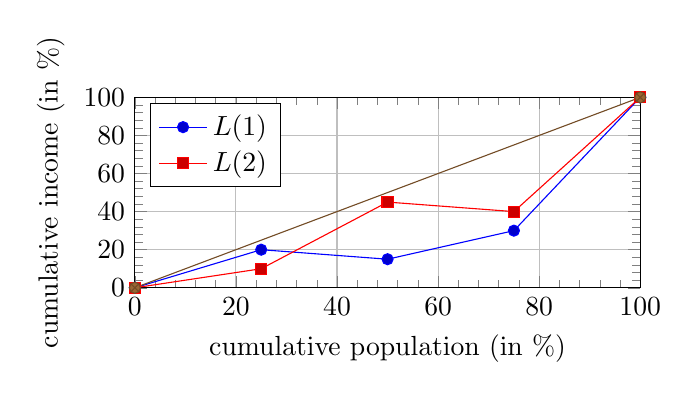
\begin{tikzpicture}
		\begin{axis}[
				xmin=0, xmax=100,
				ymin=0, ymax=100,
				minor tick num = 4,
				grid,
				ylabel = cumulative income (in \%),
				xlabel = cumulative population (in \%),
				legend style={legend pos=north west},
			]
			\addplot plot
			coordinates {(0,0) (25,20) (50,15) (75,30) (100,100)};
			\addplot plot
			coordinates {(0,0) (25,10) (50,45) (75,40) (100,100)};
			\addplot plot [thin]
			coordinates {(0,0) (100,100)};
			\legend{$L(1)$,$L(2)$}
		\end{axis}
	\end{tikzpicture}
\end{frame}

\begin{frame}{Gini Index (CART, IBM IntelligentMiner) (III)}
	\begin{itemize}
		\item Measured impurity of partition $D$ is defined as the sum over $n$ classes:
		      \begin{align*}
			      \text{Gini}(D) = 1-\sum_{j=1}^{n} p_j^2,
		      \end{align*}
		      where $p_j$ is the non-zero probability that sample in $D$ belongs to class $C_j$ as estimated by $\frac{|C_{j,D}|}{|D|}$
		\item If \textbf{attribute $A$ is discrete-valued} with $v$ distinct values
		      compute all possible subsets of values $2^v - 2$. Compute weighted sum of
		      each partition tuple ($D_1$ and $D_2$) as follows:
		      \begin{align*}
			      \text{Gini}_A(D) = \frac{|D_1|}{|D|}\text{Gini}(D_1)+\frac{|D_2|}{|D|}\text{Gini}(D_2).
		      \end{align*}
		\item If \textbf{attribute $A$ is continuous-valued} proceed similarly as in
		      calculating Information Gain for continuous-valued attributes (order values,
		      calculate midpoint of value pairs) and then calculate $\text{Gini}_A(D)$ for
		      every split point.
	\end{itemize}
\end{frame}

\begin{frame}{Gini Index (CART, IBM IntelligentMiner) (IV)}
	\begin{itemize}
		\item Gini Index as the \textbf{reduction in impurity} is then given as
		      follows:
		      \begin{align*}
			      \Delta\text{Gini}_A(D) = \text{Gini}(D)-\text{Gini}_A(D).
		      \end{align*}
		\item Attribute with minimum Gini Index is used as the splitting attribute.
	\end{itemize}

\end{frame}

\begin{frame}{Gini Index - Example (I)}
	\begin{itemize}
		\item $D$ has $9$ tuples in $\text{buys\_computer} =$ "yes" and 5 in "no", thus
		      \begin{align*}
			      \text{Gini}(D) = 1 - \left( \frac{9}{14} \right)^2 - \left( \frac{5}{14} \right)^2 = 0.459.
		      \end{align*}
		\item Suppose the attribute $\texttt{income}$ partitions $D$ \\ into $10$ in
		      $D_1:\{\texttt{low,medium}\}$ and $4$ in $D_2: \{\texttt{high}\}$:
		      \begin{align*}
			       & \text{Gini}(D\vert_{D[\texttt{income}]="medium", "low"})                                                                                                                                   \\
			       & = \frac{10}{14} \text{Gini}(D_1) + \frac{4}{14} \text{Gini}(D_2)                                                                                                                           \\
			       & =\frac{10}{14} \left(1-\left( \frac{7}{10} \right)^2 - \left( \frac{3}{10} \right)^2 \right) + \frac{4}{14} \left( 1-\left( \frac{2}{4} \right)^2 - \left( \frac{2}{4} \right)^2 \right) = \\
			       & = 0.443 = \text{gini}(D\vert_{D[\texttt{income}]="high"}).
		      \end{align*}
	\end{itemize}
\end{frame}

\begin{frame}{Gini Index - Example (II)}
	\begin{itemize}
		\item $\text{Gini}(D\vert_{D[\texttt{income}]="low", "high"}) = 0.458$,\\
		      $\text{Gini}(D\vert_{D[\texttt{income}]="medium", "high"}) = 0.450.$
		\item Thus, split on the \{"low","medium"\} and \{"high"\}, since it has the lowest gini index.
	\end{itemize}
\end{frame}

\begin{frame}{Attribute Selection Methods Overview}
	\textbf{The three methods, in general, return good results, but}
	\begin{itemize}
		\item \textbf{\color{airforceblue}Information gain:}
		      \begin{itemize}
			      \item Biased towards multi-valued attributes.
		      \end{itemize}
		\item \textbf{\color{airforceblue}Gain ratio:}
		      \begin{itemize}
			      \item Tends to prefer unbalanced splits in which one partition is much smaller than the others.
		      \end{itemize}
		\item \textbf{\color{airforceblue}Gini index:}
		      \begin{itemize}
			      \item Biased to multi-valued attributes.
			      \item Has difficulty when number of classes is large.
			      \item Tends to favor tests that result in equal-sized partitions and purity in both partitions.
		      \end{itemize}
	\end{itemize}
\end{frame}

\begin{frame}{Other Attribute Selection Methods}
	\begin{itemize}
		\item \textbf{CHAID:}
		      \begin{itemize}
			      \item A popular decision tree algorithm, measure based on $\chi^2$ test for independence.
		      \end{itemize}
		\item \textbf{C-SEP:}
		      \begin{itemize}
			      \item Performs better than Information Gain and Gini Index in certain cases.
		      \end{itemize}
		\item \textbf{G-statistic:}
		      \begin{itemize}
			      \item Has a close approximation to $\chi^2$ distribution.
		      \end{itemize}
		\item \textbf{MDL (Minimal Description Length) principle:}
		      \begin{itemize}
			      \item I.e. the simplest solution is preferred.
			      \item The best tree is the one that requires the fewest number of bits to both (1) encode the tree and (2) encode the exceptions to the tree.
		      \end{itemize}
		\item \textbf{Multivariate splits:}
		      \begin{itemize}
			      \item Partitioning based on multiple variable combinations.
			      \item CART: finds multivariate splits based on a linear combination of attributes.
		      \end{itemize}
		\item \textbf{Which Attribute Selection Method is the best?}
		      \begin{itemize}
			      \item Most give good results, none is significantly superior to others.
		      \end{itemize}
	\end{itemize}
\end{frame}

\begin{frame}{Overfitting and Tree Pruning}
	\begin{itemize}
		\item \textbf{Overfitting: An induced tree may overfit the training data.}
		      \begin{itemize}
			      \item Too many branches, some may reflect anomalies due to noise or outliers.
			      \item Poor accuracy for unseen samples.
		      \end{itemize}
		\item Pruned trees are typically smaller, less complex, easier to
		      comprehend, faster and better at classifying unseen data.
		\item \textbf{Two approaches to avoid overfitting:}
		      \begin{enumerate}
			      \item \textbf{\color{airforceblue}Prepruning:}
			            \begin{itemize}
				            \item Halt tree construction early.\\
				                  Do not split a node, if this would result in the goodness measure falling below a threshold.
				            \item Difficult to choose an appropriate threshold.
			            \end{itemize}
			      \item \textbf{\color{airforceblue}Postpruning:}
			            \begin{itemize}
				            \item Remove branches from a "fully grown" tree.\\
				                  Get a sequence of progressively pruned trees.
				            \item Use a set of data different from the training data to decide which is the "best pruned tree."
			            \end{itemize}
		      \end{enumerate}
	\end{itemize}
\end{frame}

\begin{frame}{Enhancements to Basic Decision Tree Induction}
	\begin{itemize}
		\item \textbf{Allow for} \textbf{\color{airforceblue}continuous-valued attributes.}
		      \begin{itemize}
			      \item Dynamically define new discrete-valued attributes that partition the values of continuous-valued attributes into a discrete set of intervals.
		      \end{itemize}
		\item \textbf{Handle} \textbf{\color{airforceblue}missing attribute values.}
		      \begin{itemize}
			      \item Assign the most common value of the attribute.
			      \item Assign probability to each of the possible values.
		      \end{itemize}
		\item \textbf{\color{airforceblue}Attribute construction.}
		      \begin{itemize}
			      \item Create new attributes based on existing ones that are sparsely represented.
			      \item This reduces fragmentation, repetition, and replication.
		      \end{itemize}
	\end{itemize}
\end{frame}

\begin{frame}{Classification in Large Databases}
	\begin{itemize}
		\item ID3, C4.5, and CART have been developed with the assumption that data fits into memory.\\With Big Data that's not possible anymore.
		\item \textbf{Scalability:}
		      \begin{itemize}
			      \item Classifying datasets with millions of examples and \\ hundreds of attributes with reasonable speed.
		      \end{itemize}
		\item \textbf{Why is decision tree induction popular?}
		      \begin{itemize}
			      \item Relatively fast learning speed (compared to other classification methods).
			      \item Convertible to simple and easy-to-understand classification rules.
			      \item Can use SQL queries for accessing databases.
			      \item Classification accuracy comparable with other methods.
		      \end{itemize}
		\item Two scalable methods, among others:
		      \begin{enumerate}
			      \item RainForest
			      \item BOAT
		      \end{enumerate}
	\end{itemize}
\end{frame}

\begin{frame}{Scalable Decision Tree: RainForest}
	\begin{itemize}
		\item Applicable to any decision tree algorithm.
		\item \textbf{Separates the scalability aspects from the criteria that determine the quality of the tree.}
		\item \textbf{Builds an} \textbf{\color{airforceblue}AVC-list:} (Attribute, Value, Class\_label).
		\item \textbf{\color{airforceblue}AVC-set} \textbf{(of an attribute X):}
		      \begin{itemize}
			      \item Projection of training dataset onto the attribute $X$ and class label where counts of individual class label are aggregated.
		      \end{itemize}
		\item \textbf{\color{airforceblue}AVC-group} \textbf{(of a node n):}
		      \begin{itemize}
			      \item Set of AVC-sets of all predictor attributes at the node $n$.
		      \end{itemize}
	\end{itemize}
\end{frame}

\begin{frame}{RainForest: Training Set and its AVC-sets}
	\begin{columns}
		\begin{column}{0.6\textwidth}
			\small
			\begin{tabular}{|l|l|c|c|c|}
	\hline
	\rowcolor{faugray!62}\textbf{age} & \textbf{income} & \textbf{student} & \textbf{credit\_rating} & \textbf{buys\_computer} \\\hline
	$\leq 30$                         & high            & no               & fair                    & {\color{faured}no}      \\\hline
	$\leq 30$                         & high            & no               & excellent               & {\color{faured}no}      \\\hline
	$31\ldots40$                      & high            & no               & fair                    & {\color{faugreen}yes}   \\\hline
	$>40$                             & medium          & no               & fair                    & {\color{faugreen}yes}   \\\hline
	$>40$                             & low             & yes              & fair                    & {\color{faugreen}yes}   \\\hline
	$>40$                             & low             & yes              & excellent               & {\color{faured}no}      \\\hline
	$31\ldots40$                      & low             & yes              & excellent               & {\color{faugreen}yes}   \\\hline
	$\leq 30$                         & medium          & no               & fair                    & {\color{faured}no}      \\\hline
	$\leq 30$                         & low             & no               & fair                    & {\color{faugreen}yes}   \\\hline
	$>40$                             & medium          & yes              & fair                    & {\color{faugreen}yes}   \\\hline
	$\leq 30$                         & medium          & yes              & excellent               & {\color{faugreen}yes}   \\\hline
	$31\ldots40$                      & medium          & no               & excellent               & {\color{faugreen}yes}   \\\hline
	$31\ldots40$                      & high            & yes              & fair                    & {\color{faugreen}yes}   \\\hline
	$>40$                             & medium          & no               & excellent               & {\color{faured}no}      \\\hline
\end{tabular}

		\end{column}
		\begin{column}{0.3\textwidth}
			\vspace{-3cm}

			\centering
			AVC-set on age:\\
			\begin{tabular}{|c|c|c|}
				\hline
				age          & yes & no \\\hline
				$\leq 30$    & 2   & 3  \\\hline
				$31\ldots40$ & 4   & 0  \\\hline
				$>40$        & 3   & 2  \\\hline
			\end{tabular}\\[1cm]
			AVC-set on income:\\
			\begin{tabular}{|c|c|c|}
				\hline
				income & yes & no \\\hline
				high   & 2   & 2  \\\hline
				medium & 4   & 2  \\\hline
				low    & 3   & 1  \\\hline
			\end{tabular}
		\end{column}
	\end{columns}
\end{frame}

\begin{frame}{RainForest: Training Set and its AVC-sets (II)}
	\begin{columns}
		\begin{column}{0.6\textwidth}
			\small
			\begin{tabular}{|l|l|c|c|c|}
	\hline
	\rowcolor{faugray!62}\textbf{age} & \textbf{income} & \textbf{student} & \textbf{credit\_rating} & \textbf{buys\_computer} \\\hline
	$\leq 30$                         & high            & no               & fair                    & {\color{faured}no}      \\\hline
	$\leq 30$                         & high            & no               & excellent               & {\color{faured}no}      \\\hline
	$31\ldots40$                      & high            & no               & fair                    & {\color{faugreen}yes}   \\\hline
	$>40$                             & medium          & no               & fair                    & {\color{faugreen}yes}   \\\hline
	$>40$                             & low             & yes              & fair                    & {\color{faugreen}yes}   \\\hline
	$>40$                             & low             & yes              & excellent               & {\color{faured}no}      \\\hline
	$31\ldots40$                      & low             & yes              & excellent               & {\color{faugreen}yes}   \\\hline
	$\leq 30$                         & medium          & no               & fair                    & {\color{faured}no}      \\\hline
	$\leq 30$                         & low             & no               & fair                    & {\color{faugreen}yes}   \\\hline
	$>40$                             & medium          & yes              & fair                    & {\color{faugreen}yes}   \\\hline
	$\leq 30$                         & medium          & yes              & excellent               & {\color{faugreen}yes}   \\\hline
	$31\ldots40$                      & medium          & no               & excellent               & {\color{faugreen}yes}   \\\hline
	$31\ldots40$                      & high            & yes              & fair                    & {\color{faugreen}yes}   \\\hline
	$>40$                             & medium          & no               & excellent               & {\color{faured}no}      \\\hline
\end{tabular}

		\end{column}
		\begin{column}{0.3\textwidth}
			\vspace{-3cm}

			\centering
			AVC-set on student:\\
			\begin{tabular}{|c|c|c|}
				\hline
				student & yes & no \\\hline
				yes     & 6   & 1  \\\hline
				no      & 3   & 4  \\\hline
			\end{tabular}\\[1cm]
			AVC-set on credit\_rating:\\
			\begin{tabular}{|c|c|c|}
				\hline
				credit\_rating & yes & no \\\hline
				fair           & 6   & 2  \\\hline
				excellent      & 3   & 3  \\\hline
			\end{tabular}
		\end{column}
	\end{columns}
\end{frame}

\begin{frame}{Scalable Decision Tree: BOAT}
	\begin{itemize}
		\item BOAT = Bootstrapped Optimistic Algorithm for Tree Construction
		\item \textbf{Use a statistical technique called bootstrapping to create several smaller samples (subsets), each fitting in memory.}
		      \begin{itemize}
			      \item See on the subsequent slides.
		      \end{itemize}
		\item \textbf{Each subset is used to create a tree, resulting in several trees.}
		\item \textbf{These trees are examined and used to construct a new tree T'.}
		      \begin{itemize}
			      \item It turns out that T' is very close to the tree that would be generated \\
			            using the whole data set together.
		      \end{itemize}
		\item \textbf{Advantages:}
		      \begin{itemize}
			      \item Requires only two scans of DB.
			      \item An incremental algorithm:
			            \begin{itemize}
				            \item Take insertions and deletions of training data and update the decision tree.
			            \end{itemize}
		      \end{itemize}
	\end{itemize}
\end{frame}

\begin{frame}{Presentation of Classification Results}
	\centering
	\includegraphics[height=0.8\textheight]{img/classification1.jpeg}
\end{frame}

\begin{frame}{Visualization of a Decision Tree}
	\centering
	\includegraphics[height=0.8\textheight]{img/classification2.jpeg}
\end{frame}

\begin{frame}{Interactive Visual Mining}
	\centering
	\includegraphics[height=0.8\textheight]{img/classification3.jpeg}
\end{frame}

\section{Rule-Based Classification}

\begin{frame}{Using \uppercase{if-then} Rules for Classification}
	\begin{itemize}
		\item \textbf{Represent the knowledge in the form of {\color{airforceblue}IF-THEN rules}.}
		      \begin{itemize}
			      \item E.g., if \texttt{age} $\leq 30$ AND \texttt{student} = "yes" THEN buys\_computer = "yes".
			      \item Readable.
		      \end{itemize}
		\item \textbf{Rule {\color{airforceblue}antecedent/precondition} vs. rule {\color{airforceblue}consequent}}.
		\item \textbf{Assessment of a rule R: coverage and accuracy.}
		      \begin{itemize}
			      \item $n_{\text{covers}} = \#$ of tuples covered by $R$ (antecedent if true).
			      \item $n_{\text{correct}} = \#$ of tuples correctly classified by $R$.
			      \item $\text{coverage}(R) = \frac{n_{\text{covers}}}{|D|}$ with $D$ training data set.
			      \item $\text{accuracy}(R) = \frac{n_{\text{correct}}}{n_{\text{covers}}}$.
		      \end{itemize}
	\end{itemize}
\end{frame}

\begin{frame}[c]{Potential Problems of Rule-based Classification}
	\centering
	\huge
	\begin{enumerate}
		\item More than one rule is triggered.
		\item No rule is triggered.
	\end{enumerate}
\end{frame}

\begin{frame}{Potential Problems of Rule-based Classification: Solutions}
	\begin{enumerate}
		\item \textbf{More than one rule is triggered: {\color{airforceblue}conflict resolution}.}
		      \begin{itemize}
			      \item \textbf{\color{airforceblue}Size ordering:}
			            \begin{itemize}
				            \item Assign the highest priority to the triggered rule that has the "toughest" requirement \\ (i.e., rule with most used attribute in condition).
			            \end{itemize}
			      \item \textbf{\color{airforceblue}Class-based ordering:}
			            \begin{itemize}
				            \item Decreasing order of prevalence or misclassification cost per class.
				            \item No order of rules within class $\rightarrow$ disjunction (logical \texttt{OR}) between rules.
			            \end{itemize}
			      \item \textbf{\color{airforceblue}Rule-based ordering} (decision list):
			            \begin{itemize}
				            \item Rules are organized into one long priority list,\\
				                  according to some measure of rule quality, or by experts.
				            \item Rules \underline{must} be applied in this particular order to avoid conflict.
			            \end{itemize}
		      \end{itemize}
		\item \textbf{No rule is triggered.}
		      \begin{itemize}
			      \item Use a fallback/default rule.
			      \item Always evaluated as the last rule, if and only if other rules are not covered by some tuple, i. e. no rules have been triggered.
		      \end{itemize}
	\end{enumerate}
\end{frame}

\begin{frame}{Rule Extraction from a Decision Tree}
	\begin{itemize}
		\item \textbf{Rules are {\color{airforceblue}easier to understand} than large trees.}
		\item \textbf{Rule can be created for {\color{airforceblue}each path from the root to a leaf.}}
		      \begin{itemize}
			      \item The leaf holds the class prediction.
		      \end{itemize}
		\item \textbf{Each attribute-value pair along the path forms a conjunction:}
	\end{itemize}
	\vspace*{1em}
	\begin{columns}
		\begin{column}{0.7\textwidth}
			\textbf{Example:}
			\begin{enumerate}
				\item IF \texttt{age} $\leq$ 30 AND \texttt{student} = "no" \\
				      THEN \texttt{buys\_computer} = "no".
				\item IF \texttt{age} $\leq$ 30 AND \texttt{student} = "yes" \\
				      THEN \texttt{buys\_computer} = "yes".
				\item IF \texttt{age}== $31\ldots40$ THEN \texttt{buys\_computer} = "yes".
				\item \dots
			\end{enumerate}
		\end{column}
		\begin{column}{0.3\textwidth}
			\begin{figure}[h]
				\centering
				\begin{tikzpicture}[
		overlay,
		remember picture,
		>=latex,
		thick,
		node/.style={
				draw=faugray,
				rounded corners=.25em,
				fill=faugray!62,
				text depth=0.2em
			},
		leaf/.style={
				draw,
				rounded corners=.7em,
				text depth=0.2em
			},
		branch/.style={
				fill=white,
				font=\ttfamily\scriptsize,
				rounded corners=.7em,
				text depth=0.2em
			}
	]
	\node[node] at (0,0) (age) {age?};
	\node[leaf,text=faugreen,below=6.2em of age] (age-yes) {yes};

	\node[node,below left=2em and 1.5em of age] (student) {student?};
	\node[leaf,text=faured,below right=2.5em and -1em of student] (student-no) {no};
	\node[leaf,text=faugreen,below left=2.5em and -1em of student] (student-yes) {yes};

	\node[node,below right=2em and .6em of age] (credit-rating) {credit rating?};
	\node[leaf,text=faured,below left=2.5em and -2em of credit-rating] (credit-no) {no};
	\node[leaf,text=faugreen,below right=2.5em and -2em of credit-rating] (credit-yes) {yes};

	\draw (age.south) -- (age-yes.north);
	\node[branch,below=4em of age.north] {31\dots 40};

	\draw[rounded corners=5pt]
	(age.south) -- ($(age.south) + (0,-1em)$) --
	($(student.north) + (0,1em)$) -- (student.north);
	\node[branch,above=1em of student.north] {$\leq$30};

	\path[draw,rounded corners=5pt]
	(age.south) -- ($(age.south) + (0,-1em)$) --
	($(credit-rating.north) + (0,1em)$) -- (credit-rating.north);
	\node[branch,above=1em of credit-rating.north] {>40};

	% student labels
	\draw[rounded corners=5pt]
	(student.south) -- ($(student.south) + (0,-1.5em)$) --
	($(student-no.north) + (0,1em)$) -- (student-no.north);
	\node[branch,above=1em of student-no.north] {no};

	\draw[rounded corners=5pt]
	(student.south) -- ($(student.south) + (0,-1.5em)$) --
	($(student-yes.north) + (0,1em)$) -- (student-yes.north);
	\node[branch,above=1em of student-yes.north] {yes};

	% credit-rating labels
	\draw[rounded corners=5pt]
	(credit-rating.south) -- ($(credit-rating.south) + (0,-1.5em)$) --
	($(credit-no.north) + (0,1em)$) -- (credit-no.north);
	\node[branch,above=1em of credit-no.north] {excellent};

	\draw[rounded corners=5pt]
	(credit-rating.south) -- ($(credit-rating.south) + (0,-1.5em)$) --
	($(credit-yes.north) + (0,1em)$) -- (credit-yes.north);
	\node[branch,above=1em of credit-yes.north] {fair};
\end{tikzpicture}

			\end{figure}
		\end{column}
	\end{columns}
\end{frame}

\begin{frame}{Rule Induction: Sequential Covering Method}
	\begin{itemize}
		\item \textbf{Sequential covering algorithm:}
		      \begin{itemize}
			      \item Extracts rules directly from training data.
		      \end{itemize}
		\item \textbf{Typical sequential covering algorithms:}
		      \begin{itemize}
			      \item FOIL, AQ, CN2, RIPPER.
		      \end{itemize}
		\item \textbf{Rules are learned {\color{airforceblue}sequentially}.}
		      \begin{itemize}
			      \item Each rule for a given class $C_i$ will cover many tuples of $C_i$, but none (or few) of the tuples of other classes.
		      \end{itemize}
		\item \textbf{Algorithm sketch:}
		      \begin{itemize}
			      \item Rules are learned one at a time.
			      \item Each time a rule is learned, the tuples covered by the rule are removed.
			      \item The process repeats on the remaining tuples unless termination condition, e.g., when no more training examples left or when the quality of a rule returned is below a user-specified threshold.
		      \end{itemize}
		\item \textbf{Compare with decision-tree induction:}
		      \begin{itemize}
			      \item That was learning a set of rules simultaneously.
		      \end{itemize}
	\end{itemize}
\end{frame}

\begin{frame}{Sequential Covering Algorithm}
	\begin{itemize}
		\item \textbf{While (enough target tuples left):}
		      \begin{itemize}
			      \item generate a rule;
			      \item remove positive target tuples satisfying this rule;
		      \end{itemize}
		      \centering
		      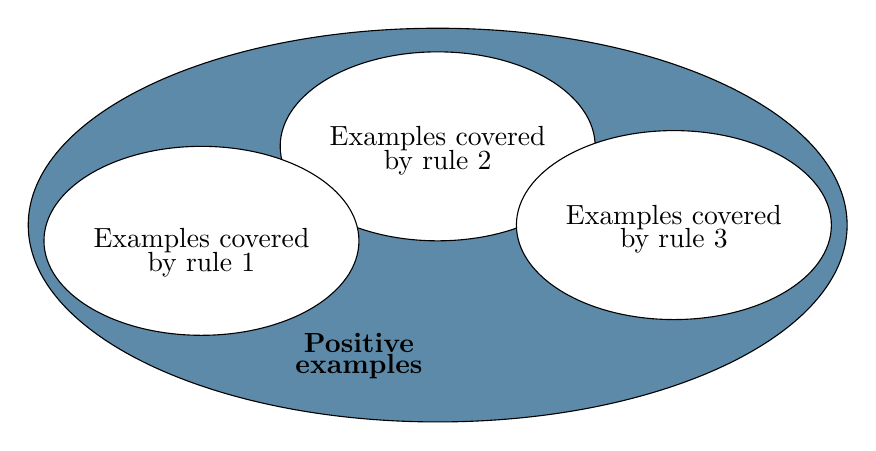
\begin{tikzpicture}
			      \draw[fill=airforceblue] (0,0) ellipse (5.2 and 2.5) (0,0) node [text=black] {};
			      \draw[fill=white] (0,1) ellipse (2 and 1.2) (0,0) node [text=black] {};
			      \draw[fill=white] (-3,-0.2) ellipse (2 and 1.2) (0,0) node [text=black] {};
			      \draw[fill=white] (3,0) ellipse (2 and 1.2) (0,0) node [text=black] {};
			      \node at (0,1.1) (a1) {Examples covered};
			      \node at (0,0.8) (a2) {by rule 2};
			      \node at (3,0.1) (b1) {Examples covered};
			      \node at (3,-0.2) (b2) {by rule 3};
			      \node at (-3,-0.2) (c1) {Examples covered};
			      \node at (-3,-0.5) (c2) {by rule 1};
			      \node at (-1,-1.5) (d1) {\textbf{Positive}};
			      \node at (-1,-1.8) (d2) {\textbf{examples}};
		      \end{tikzpicture}
	\end{itemize}
\end{frame}

\begin{frame}{Sequential Covering Algorithm (II)}
	\begin{itemize}
		\item \textbf{To generate a rule:}
		      \begin{itemize}
			      \item \textbf{while}(true:)
			            \begin{itemize}
				            \item find the best predicate $p$ (attribute = value);
				            \item \textbf{if} \texttt{FOIL\_Gain}(p) > threshold
				            \item \textbf{then} add $p$ to current rule;
				            \item \textbf{else} break;
			            \end{itemize}
		      \end{itemize}
	\end{itemize}
	\centering
	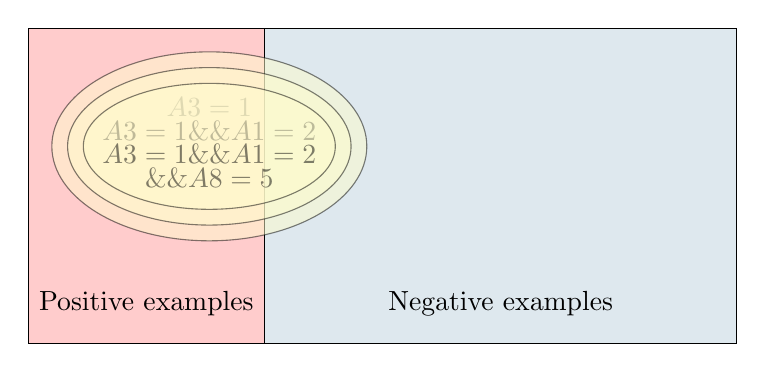
\begin{tikzpicture}
		\draw[fill=red!20] (-3,0) rectangle (1,4) (0,0) node [text=black] {};
		\draw[fill=airforceblue!20] (6,0) rectangle (0,4) (0,0) node [text=black] {};
		\node at (3,0.5) (a1) {Negative examples};
		\node at (-1.5,0.5) (a1) {Positive examples};
		\draw[fill=yellow!20, opacity=0.5] (-0.7,2.5) ellipse (2 and 1.2) (0,0) node [text=black] {};
		\node[opacity=0.5] at (-0.7,3) {$A3=1$};
		\draw[fill=yellow!20, opacity=0.5] (-0.7,2.5) ellipse (1.8 and 1) (0,0) node [text=black] {};
		\node[opacity=0.5] at (-0.7,2.7) {$A3=1 \&\& A1=2$};
		\draw[fill=yellow!20, opacity=0.5] (-0.7,2.5) ellipse (1.6 and 0.8) (0,0) node [text=black] {};
		\node[opacity=0.5] at (-0.7,2.4) {$A3=1 \&\& A1=2$};
		\node[opacity=0.5] at (-0.7,2.1) {$\&\& A8=5$};
	\end{tikzpicture}
\end{frame}

% TODO: Review again and cosmetics
\begin{frame}{Sequential Covering Algorithm (III)}
	\begin{itemize}
		\item \textbf{Start with the most general rule possible:}
		      \begin{itemize}
			      \item Condition = empty.
		      \end{itemize}
		\item \textbf{Add new attributes by adopting a greedy depth-first strategy.}
		      \begin{itemize}
			      \item Pick the one that improves the rule quality most.
			      \item Current rule $R$: IF condition THEN class = c.
			      \item New rule $R'$: IF condition' THEN class = c,
			      \item $pos/neg$ are $\#$ of positive/negative tuples covered by $R$.
		      \end{itemize}
		\item \textbf{Rule-quality measures.}
		      \begin{itemize}
			      \item Must consider both coverage and accuracy.
			      \item \texttt{FOIL\_Gain} (from \texttt{FOIL} - First-Order Inductive Learner):
			            \begin{align}
				            \text{FOIL\_Gain} = \text{pos}' \left( \log_2 \frac{\text{pos}'}{\text{pos}' + \text{neg}'} - \log_2 \frac{\text{pos}}{\text{pos}+\text{neg}} \right).
			            \end{align}
			      \item Favors rules that have high accuracy and cover many positive tuples.
		      \end{itemize}
	\end{itemize}
\end{frame}

\begin{frame}{Rule Pruning}
	\begin{itemize}
		\item \textbf{Danger of {\color{airforceblue}overfitting}.}
		\item \textbf{Removing a conjunct (attribute test),}
		      \begin{itemize}
			      \item if pruned version of rule has greater quality,\\
			            assessed on an independent set of test tuples (called "pruning set").
		      \end{itemize}
		\item \textbf{FOIL uses:}
		      \begin{align}
			      \text{FOIL\_Prune}(R) = \frac{\text{pos}-\text{neg}}{\text{pos}+\text{neg}}.
		      \end{align}
		\item If $\text{FOIL\_Prune}$ is higher for the pruned version of $R$, prune $R$.
	\end{itemize}
\end{frame}

\section{Bayes Classification Methods}

\begin{frame}{Bayesian Classification: Why?}
	\begin{itemize}
		\item \textbf{A statistical classifier:}
		      \begin{itemize}
			      \item Performs probabilistic prediction, i.e. predicts class-membership probabilities.
		      \end{itemize}
		\item \textbf{Foundation:} \textbf{\color{airforceblue}Bayes' Theorem.}
		\item \textbf{Performance:}
		      \begin{itemize}
			      \item A simple Bayesian classifier (naïve Bayesian classifier) has performance comparable with decision tree and selected neural-network classifiers.
		      \end{itemize}
		\item \textbf{Incremental:}
		      \begin{itemize}
			      \item Each training example can incrementally increase/decrease the probability that a hypothesis is correct -- prior knowledge can be combined with observed data.
		      \end{itemize}
		\item \textbf{Standard:}
		      \begin{itemize}
			      \item Even when Bayesian methods are computationally intractable, they can provide a standard of optimal decision making against which other methods can be measured.
		      \end{itemize}
	\end{itemize}
\end{frame}

\begin{frame}{Bayes' Theorem: Basics}
	\begin{itemize}
		\item \textbf{Let $X$ be a data sample ("evidence").}
		      \begin{itemize}
			      \item The class label shall be unknown.
		      \end{itemize}
		\item \textbf{Let $C_i$ be the hypothesis that $X$ belongs to class $i$.}
		\item \textbf{Classification is to determine $P(C_i|X)$:}
		      \begin{itemize}
			      \item \textbf{\color{airforceblue}Posteriori probability:} the probability that the hypothesis \\ holds given the observed data sample $X$.
		      \end{itemize}
		\item $P(C_i)$:
		      \begin{itemize}
			      \item \textbf{\color{airforceblue}Prior probability:} the initial probability.
			      \item E.g., $X$ will buy computer, regardless of age, income, $\ldots$
		      \end{itemize}
		\item $P(X)$:
		      \begin{itemize}
			      \item Probability that sample data is observed.
		      \end{itemize}
		\item $P(X|C_j)$:
		      \begin{itemize}
			      \item \textbf{\color{airforceblue}Likelihood:} the probability of observing the sample $X$ given that the hypothesis holds.
			      \item E.g., given that $X$ buys computer, the probability that $X$ is $31\ldots40$, medium income.
		      \end{itemize}
	\end{itemize}
\end{frame}

\begin{frame}{Bayes' Theorem (II)}
	\begin{itemize}
		\item \textbf{Given training data $X$, the posteriori probability $P(C_i|X)$\\
			      of a hypothesis $C_i$ follows from the Bayes' Theorem:}
		      \begin{align}
			      P(C_i|X) = \frac{P(X|C_i)P(C_i)}{P(X)}.
		      \end{align}
		\item \textbf{Predicts that $X$ belongs to $C_i$ if the probability $P(C_i|X)$\\
			      is {\color{airforceblue}the highest} among all the $P(C_k|X)$ for all $k$ classes.}
		\item \textbf{Practical difficulty:}
		      \begin{itemize}
			      \item Requires initial knowledge of many probabilities.
			      \item Significant computational cost.
		      \end{itemize}
	\end{itemize}
\end{frame}

\begin{frame}{Towards Naïve Bayesian Classifier}
	\begin{itemize}
		\item \textbf{Let $D$ be a training set of tuples and their associated class labels.}
		      \begin{itemize}
			      \item Each tuple is represented by an $n$-dimensional attribute $X = (x_1,x_2,\ldots,x_n)$.
		      \end{itemize}
		\item \textbf{Supose there are $m$ classes $C_1,C_2, \ldots, C_m$.}
		\item \textbf{Classification is to derive the {\color{airforceblue}maximum posteriori probability}.}
		      \begin{itemize}
			      \item i.e. the maximal $P(C_i|X)$.
		      \end{itemize}
		\item \textbf{This can be derived from Bayes' Theorem:}
		      \begin{align}
			      P(C_i|X) = \frac{P(X|C_i)P(C_i)}{P(X)}.
		      \end{align}
		\item \textbf{Since $P(X)$ is constant for all classes, we must maximize only:}
		      \begin{align}
			      P(X|C_i)P(C_i).
		      \end{align}
	\end{itemize}
\end{frame}

\begin{frame}{Derivation of Naïve Bayes Classifier}
	\begin{itemize}
		\item \textbf{A simplifying assumption: attributes are {\color{airforceblue}conditionally independent}.}
		      \begin{itemize}
			      \item I.e. no dependence relation between attributes (which is "naïve").
			            \begin{align*}
				            \resizebox{7cm}{!}{%
					            $P(X|C_i) = \prod_{k=1}^{n} P(x_k|C_i) = P(x_1|C_i)P(x_2|C_i)\cdots P(x_n|C_i).$}
			            \end{align*}
			      \item This greatly reduces the computation cost:\\
			            Only count the class distribution.
			      \item If $A_k$ is categorical,
			            \begin{itemize}
				            \item $P(x_k|C_i)$is the number of tuples in $C_i$ having value $x_k$ for $A_k$ \\
				                  divided by $|C_{i,D}|$ (the number of tuples of $C_i$ in $D$).
			            \end{itemize}
			      \item If $A_k$ is continuous-valued,
			            \begin{itemize}
				            \item $P(x_k|C_i)$ is usually computed based on Gaussian distribution with a mean $\mu$ and standard deviation $\sigma$:
				                  \begin{align*}
					                  \resizebox{4cm}{!}{%
					                  $G(x,\mu,\sigma) = \frac{1}{\sqrt{2\pi}\sigma}e^{\frac{(x-\mu)^2}{2\sigma^2}},$}
				                  \end{align*}
				            \item and $P(x_k|C_i) = G(x_k,\mu_{C_i},\sigma_{C_i})$.
			            \end{itemize}
		      \end{itemize}
	\end{itemize}
\end{frame}

\begin{frame}{Naïve Bayesian Cellcolormake Dataset}
	\begin{columns}
		\begin{column}{0.4\textwidth}
			\vspace{-2cm}
			\begin{itemize}
				\item \textbf{Classes:}
				      \begin{itemize}
					      \item $C_1$: \texttt{buys\_computer} = "yes".
					      \item $C_2$: \texttt{buys\_computer} = "no".
				      \end{itemize}
				\item \textbf{Data sample:}
				      \begin{itemize}
					      \item $X = (\texttt{age} \leq 30,$ \\
					            $\texttt{income} = "medium",$ \\
					            $\texttt{student} = "yes",$\\
					            $\texttt{credit\_rating} = "fair")$.
				      \end{itemize}
			\end{itemize}
		\end{column}
		\begin{column}{0.6\textwidth}
			\resizebox{\columnwidth}{!}{%
				\begin{tabular}{|l|l|c|l|c|}
					\hline
					\cellcolor{blue!20}age            & \cellcolor{blue!20}income   & \cellcolor{blue!20}student & \cellcolor{blue!20}credit\_rating & \cellcolor{brown!20}buys\_computer \\\hline
					\cellcolor{yellow!20}$\leq30$     & \cellcolor{yellow!20}high   & \cellcolor{yellow!20}no    & \cellcolor{yellow!20}fair         & \cellcolor{red!20}no               \\\hline
					\cellcolor{yellow!20}$\leq30$     & \cellcolor{yellow!20}high   & \cellcolor{yellow!20}no    & \cellcolor{yellow!20}excellent    & \cellcolor{red!20}no               \\\hline
					\cellcolor{yellow!20}$31\ldots40$ & \cellcolor{yellow!20}high   & \cellcolor{yellow!20}no    & \cellcolor{yellow!20}fair         & \cellcolor{green!20}yes            \\\hline
					\cellcolor{yellow!20}$>40$        & \cellcolor{yellow!20}medium & \cellcolor{yellow!20}no    & \cellcolor{yellow!20}fair         & \cellcolor{green!20}yes            \\\hline
					\cellcolor{yellow!20}$>40$        & \cellcolor{yellow!20}low    & \cellcolor{yellow!20}yes   & \cellcolor{yellow!20}fair         & \cellcolor{green!20}yes            \\\hline
					\cellcolor{yellow!20}$>40$        & \cellcolor{yellow!20}low    & \cellcolor{yellow!20}yes   & \cellcolor{yellow!20}excellent    & \cellcolor{red!20}no               \\\hline
					\cellcolor{yellow!20}$31\ldots40$ & \cellcolor{yellow!20}low    & \cellcolor{yellow!20}yes   & \cellcolor{yellow!20}excellent    & \cellcolor{green!20}yes            \\\hline
					\cellcolor{yellow!20}$\leq30$     & \cellcolor{yellow!20}medium & \cellcolor{yellow!20}no    & \cellcolor{yellow!20}fair         & \cellcolor{red!20}no               \\\hline
					\cellcolor{yellow!20}$>40$        & \cellcolor{yellow!20}medium & \cellcolor{yellow!20}yes   & \cellcolor{yellow!20}fair         & \cellcolor{green!20}yes            \\\hline
					\cellcolor{yellow!20}$\leq30$     & \cellcolor{yellow!20}medium & \cellcolor{yellow!20}yes   & \cellcolor{yellow!20}excellent    & \cellcolor{green!20}yes            \\\hline
					\cellcolor{yellow!20}$31\ldots40$ & \cellcolor{yellow!20}medium & \cellcolor{yellow!20}no    & \cellcolor{yellow!20}fair         & \cellcolor{green!20}yes            \\\hline
					\cellcolor{yellow!20}$31\ldots40$ & \cellcolor{yellow!20}high   & \cellcolor{yellow!20}yes   & \cellcolor{yellow!20}fair         & \cellcolor{green!20}yes            \\\hline
					\cellcolor{yellow!20}$>40$        & \cellcolor{yellow!20}medium & \cellcolor{yellow!20}no    & \cellcolor{yellow!20}excellent    & \cellcolor{red!20}no               \\\hline
				\end{tabular}}
		\end{column}
	\end{columns}
\end{frame}

\begin{frame}{Naïve Bayesian Classifier: An Example}
	\begin{itemize}
		\item $P(C_i)$:
		      \begin{itemize}
			      \item $P(\texttt{buys\_computer} = "yes") = \frac{9}{14} = 0.643$.
			      \item $P(\texttt{buys\_computer} = "no") = \frac{5}{14} = 0.357$.
		      \end{itemize}
		\item $X = (\texttt{age} \leq 30 , \texttt{income} = "medium", \texttt{student} = "yes", \texttt{credit\_rating} = "fair")$.
		\item \textbf{Compute $P(X|C_i)$ for each class:}
		      \begin{itemize}
			      \item $P(\texttt{age} \leq 30 | \texttt{buys\_computer} = "yes") = \frac{2}{9} = 0.222$.
			      \item $P(\texttt{age} \leq 30 | \texttt{buys\_computer} = "no") = \frac{3}{5} = 0.6$.
			      \item $P(\texttt{income} = "medium" | \texttt{buys\_computer} = "yes") = \frac{4}{9} = 0.444$.
			      \item $P(\texttt{income} = "medium" | \texttt{buys\_computer} = "no") = \frac{2}{5} = 0.4$.
			      \item $P(\texttt{student} = "yes" | \texttt{buys\_computer} = "yes") = \frac{6}{9} = 0.667$.
			      \item $P(\texttt{student} = "yes" | \texttt{buys\_computer} = "no") = \frac{1}{5} = 0.2$.
			      \item $P(\texttt{credit\_rating} = "fair" | \texttt{buys\_computer} = "yes") = \frac{6}{9} = 0.667$.
			      \item $P(\texttt{credit\_rating} = "fair" | \texttt{buys\_computer} = "no") = \frac{2}{5} = 0.4$.
		      \end{itemize}
	\end{itemize}
\end{frame}

\begin{frame}{Naïve Bayesian Classifier: An Example (II)}
	\begin{itemize}
		\item $P(C_i)$:
		      \begin{itemize}
			      \item $P(X | \texttt{buys\_computer} = "yes") = 0.222 \cdot 0.444 \cdot 0.667 \cdot 0.667 = 0.044$.
			      \item $P(X | \texttt{buys\_computer} = "no") = 0.6 \cdot 0.4 \cdot 0.2 \cdot 0.4 = 0.019$.
		      \end{itemize}
		\item $P(X | C_i) \cdot P(C_i)$:
		      \begin{itemize}
			      \item $P(X | \texttt{buys\_computer} = "yes") \cdot  P(\texttt{buys\_computer} = "yes") = 0.028$.
			      \item $P(X | \texttt{buys\_computer} = "no") \cdot  P(\texttt{buys\_computer} = "no") = 0.007$.
		      \end{itemize}
		\item \textbf{Therefore, $X$ belongs to class $C_1$ (\texttt{buys\_computer} = "yes")}.
	\end{itemize}
\end{frame}

\begin{frame}{Avoiding the Zero-probability Problem}
	\begin{itemize}
		\item \textbf{Naïve Bayesian prediction requires each conditional probability to be non-zero.}
		      \begin{itemize}
			      \item Otherwise, the predicted probability will be zero.
			            \begin{align}
				            \resizebox{4cm}{!}{
					            $P(X|C_i) = \prod_{k=1}^{n} P(x_k|C_i).$}
			            \end{align}
		      \end{itemize}
		\item \textbf{Example:}
		      \begin{itemize}
			      \item Suppose a dataset with $1000$ tuples, \texttt{income} = "low" $(0)$, \texttt{income} = "medium" $(990)$, and \texttt{income} = "high" $(10)$.
		      \end{itemize}
		\item \textbf{Use {\color{airforceblue}Laplacian correction} (or Laplacian estimator):}
		      \begin{itemize}
			      \item Add $1$ to each case:
			            \begin{itemize}
				            \item $P(\texttt{income} = "low") = \frac{1}{1003}$.
				            \item $P(\texttt{income} = "medium") = \frac{991}{1003}$.
				            \item $P(\texttt{income} = "high") = \frac{11}{1003}$.
			            \end{itemize}
			      \item The "corrected" probability estimates are close to their "uncorrected" counterparts.
		      \end{itemize}
	\end{itemize}
\end{frame}

\begin{frame}{Naïve Bayesian Classifier: Comments}
	\textbf{Advantages}
	\begin{itemize}
		\item Easy to implement.
		\item Good results obtained in most of the cases.
	\end{itemize}

	\textbf{Disadvantages}
	\begin{itemize}
		\item Assumption: class conditional independence, therefore loss of accuracy.
		\item Practically, \textbf{dependencies} exist among variables.
		      \begin{itemize}
			      \item E.g., hospital patients:
			            \begin{itemize}
				            \item Profile: age, family history, etc.
				            \item Symptoms: fever, cough, etc.
				            \item Disease: lung cancer, diabetes, etc.
			            \end{itemize}
			      \item Cannot be modeled by naïve Bayesian classifier.
		      \end{itemize}
	\end{itemize}

	\textbf{How to deal with these dependencies?} $\rightarrow$ Bayesian belief networks (see textbook).
\end{frame}

\section{Model Evaluation and Selection}\label{class:evaluation}

\begin{frame}{Model Evaluation and Selection}
	\begin{itemize}
		\item \textbf{Evaluation metrics:}
		      \begin{itemize}
			      \item How can we measure accuracy?
			      \item Other metrics to consider?
		      \end{itemize}
		\item \textbf{Use {\color{airforceblue}test} set of class-labeled tuples instead of training set when assessing accuracy.}
		\item \textbf{Methods for estimating a classifier's accuracy:}
		      \begin{itemize}
			      \item Holdout method, random subsampling.
			      \item Cross-validation.
			      \item Bootstrap.
		      \end{itemize}
		\item \textbf{Comparing classifiers:}
		      \begin{itemize}
			      \item Confidence intervals.
			      \item Cost-benefit analysis and ROC curves.
		      \end{itemize}
	\end{itemize}
\end{frame}

\begin{frame}{Confusion Matrix and Evaluation Metrics}
	Given $M$ classes, an entry $C^{(m)}_{ij}$ in an $M \times M$ confusion matrix
	indicates the number of tuples in class $i$ that were labeled by the
	classifier as class $j$.
	\begin{columns}[T]
	\begin{column}[T]{0.45\textwidth}
		\begin{tabular}{c|c|p{1cm}|p{1cm}|c|}

			\multicolumn{2}{c|}{\multirow{2}{*}{}} & \multicolumn{2}{c|}{Predicted Class} &                                           \\\cline{3-4}
			\multicolumn{2}{c|}{}                  & $C_1$                                & $\neg C_1$  & Total                       \\\hline
			\multirow{2}{*}{True Class}            & $C_1$                                & \textbf{TP} & \textbf{FN}    & \textbf{P} \\\cline{2-4}
			                                       & $\neg C_1$                           & \textbf{FP} & \textbf{TN}    & \textbf{N} \\\hline
			\multicolumn{2}{r|}{Total}             & \textbf{P'}                          & \textbf{N'} & \textbf{P + N}
		\end{tabular}

	\end{column}

	\begin{column}[T]{0.5\textwidth}
		\footnotesize
		\begin{itemize}
			\item \textbf{True Positives (TP)} = correctly classified tuples.
			\item \textbf{True Negatives (TN)} = correctly classified tuples.
			\item \textbf{False Positives (FP)} = negative tuples incorrectly classified as positive.
			\item \textbf{False Negatives (FN)} = positive tuples incorrectly classified as negative.
		\end{itemize}
		% REVIEW: I have already added the abbreviations TP, FN, FP and TN to the legend, but strictly speaking an introduction of P, N, P' and N' is still missing. Since I believe that the slides would be finally overloaded if a legend for them is added, I skip the introduction for the time being, and just leave you a note on this.
	\end{column}
\end{columns}


	\textbf{Accuracy:}
	\vspace*{-1em}
	\begin{columns}
		\begin{column}{0.55\textwidth}
			\begin{itemize}
				\item Percentage of correctly classified tuples.
				\item Also known as the (overall) recognition rate.
				\item Most effective with a \textit{balanced dataset}.
				\item Inverse: \textbf{Error rate} as the misclassification rate.
			\end{itemize}
		\end{column}
		\begin{column}{0.4\textwidth}
			\vspace*{-1.2em}
			\begin{align}
				\text{Accuracy}   & = \frac{\text{TP} + \text{TN}}{\text{P} +  \text{N}} \\
				\text{Error Rate} & = 1 - \text{Accuracy}                                \\
				                  & = \frac{\text{FP} + \text{FN}}{\text{P} + \text{N}}
			\end{align}
		\end{column}
	\end{columns}
\end{frame}

\begin{frame}{Confusion Matrix and Evaluation Metrics (II)}
	\begin{columns}[T]
	\begin{column}[T]{0.45\textwidth}
		\begin{tabular}{c|c|p{1cm}|p{1cm}|c|}

			\multicolumn{2}{c|}{\multirow{2}{*}{}} & \multicolumn{2}{c|}{Predicted Class} &                                           \\\cline{3-4}
			\multicolumn{2}{c|}{}                  & $C_1$                                & $\neg C_1$  & Total                       \\\hline
			\multirow{2}{*}{True Class}            & $C_1$                                & \textbf{TP} & \textbf{FN}    & \textbf{P} \\\cline{2-4}
			                                       & $\neg C_1$                           & \textbf{FP} & \textbf{TN}    & \textbf{N} \\\hline
			\multicolumn{2}{r|}{Total}             & \textbf{P'}                          & \textbf{N'} & \textbf{P + N}
		\end{tabular}

	\end{column}

	\begin{column}[T]{0.5\textwidth}
		\footnotesize
		\begin{itemize}
			\item \textbf{True Positives (TP)} = correctly classified tuples.
			\item \textbf{True Negatives (TN)} = correctly classified tuples.
			\item \textbf{False Positives (FP)} = negative tuples incorrectly classified as positive.
			\item \textbf{False Negatives (FN)} = positive tuples incorrectly classified as negative.
		\end{itemize}
		% REVIEW: I have already added the abbreviations TP, FN, FP and TN to the legend, but strictly speaking an introduction of P, N, P' and N' is still missing. Since I believe that the slides would be finally overloaded if a legend for them is added, I skip the introduction for the time being, and just leave you a note on this.
	\end{column}
\end{columns}

	\begin{columns}
		\begin{column}{0.4\textwidth}
			\begin{itemize}
				\item \textbf{Sensitivity} = True positive rate.
				\item \textbf{Specificity} = True negative rate.
				\item \textbf{Precision} = Measure of exactness.
				\item \textbf{Recall} = Measure of completeness.\\
				      Perfect score is 1.0.\\
				      Inverse relationship with precision.
			\end{itemize}
		\end{column}

		\begin{column}{0.6\textwidth}
			\begin{align}
				\text{Sensitivity} & = \frac{\text{TP}}{\text{P}}              & = \frac{\text{TP}}{\text{TP} + \text{FN}} & = \text{Recall} \\
				\text{Specificity} & = \frac{\text{TN}}{\text{N}}                                                                            \\
				\text{Precision}   & = \frac{\text{TP}}{\text{TP} + \text{FP}}
			\end{align}
		\end{column}
	\end{columns}
\end{frame}

\begin{frame}{Confusion Matrix and Evaluation Metrics (III)}
	\textbf{F-Measure}: Combines precision and recall in one single measure.

	\begin{columns}
		\begin{column}{0.5\textwidth}
			\begin{center}
				\textbf{$\text{\textbf{F}}_1$ Measure}
			\end{center}
			\begin{align}
				\text{F}_1 = \frac{2 \times \text{Precision} \times \text{Recall}}{\text{Precision} + \text{Recall}}
			\end{align}

			\begin{itemize}
				\item Harmonic mean between precision and recall.
				\item Equal weight to both measures.
			\end{itemize}
		\end{column}

		\begin{column}{0.5\textwidth}
			\begin{center}
				\textbf{$\text{\textbf{F}}_\beta$ Measure}
			\end{center}
			\vspace*{-.5em}
			\begin{align}
				\text{F}_\beta = \frac{(1 + \beta^2) \times \text{Precision} \times \text{Recall}}{\beta^2 \times \text{Precision} + \text{Recall}}
			\end{align}

			\begin{itemize}
				\item Weighted measure.
				\item Gives $\beta$-times more weight to precision.
			\end{itemize}
		\end{column}
	\end{columns}
\end{frame}

% TODO: Update example with confusion matrix
\begin{frame}{Example: Confusion Matrix and Evaluation Metrics (I)}
	\begin{tabular}{|c|c|c|c|}
		\hline
		Actual class/predicted class: & buys\_computer = yes & buys\_computer = no & Total \\\hline
		buys\_computer = yes          & \textbf{6954}        & \textbf{46}         & 7000  \\\hline
		buys\_computer = no           & \textbf{412}         & \textbf{2588}       & 3000  \\\hline
		Total                         & 7366                 & 2634                & 10000 \\\hline
	\end{tabular}
\end{frame}


\begin{frame}{Example: Confusion Matrix and Evaluation Metrics (II)}
	\centering
	\begin{tabular}{|c|c|c|c|c|}
		\hline
		Actual class/predicted class & cancer = yes & cancer = no   & Total & Recognition ($\%$)  \\\hline
		cancer = yes                 & \textbf{90}  & \textbf{210}  & 300   & 30.00 (sensitivity) \\\hline
		cancer = no                  & \textbf{140} & \textbf{9560} & 9700  & 98.56 (specificity) \\\hline
		Total                        & 230          & 9770          & 10000 & 96.40 (accuracy)    \\\hline
	\end{tabular}\\[0.2cm]
	\begin{itemize}
		\item Precision $= \frac{90}{230} = 39.13 \%$.
		\item Recall $=\frac{90}{300} = 30.00 \%$.
		\item $F_1$-measure = $\frac{2 \cdot 0.3913 \cdot 0.3}{0.3913 + 0.3} = 33.96 \%$.
	\end{itemize}
\end{frame}

\begin{frame}{Evaluation Strategies: Holdout Method}
	\textbf{Holdout method.}
	\begin{itemize}
		\item Randomly assign tuples into two independent sets:
		      \begin{itemize}
			      \item \textbf{\color{airforceblue}Training set} (E.g., $2/3$) for model construction.
			      \item \textbf{\color{airforceblue}Test set} (E.g., $1/3$) for accuracy estimation.
		      \end{itemize}
		\item Random sampling: a variation of holdout.
		      \begin{itemize}
			      \item Repeat holdout $k$ times, i. e. create multiple random splits and
			            multiple model construction and accuracy estimation.
			      \item Create an average accuracy over all experiments.
		      \end{itemize}
	\end{itemize}

\end{frame}

\begin{frame}{Evaluation Strategies: Cross Validation}
	Also known as $k$-fold cross validation. ($k=10$ is popular)
	\begin{columns}[T]
		\begin{column}[T]{0.5\textwidth}
			\begin{itemize}
				\item Randomly partition the data into $k$ mutually exclusive subsets (folds), each approximately equal size.
				\item At $i$-th iteration, use $D_i$ as test set and the others as training set.
				\item Average accuracy of all iterations.
				\item \textbf{Leave-one-out}: $k$ folds, on $i$-th iteration leave out $i$-th fold; for small-sized data.
				\item \textbf{Stratified cross-validation}: For every class select a simple random sample of tuples. Results in subsets with approximately the same distribution.
			\end{itemize}

		\end{column}

		\begin{column}[T]{0.5\textwidth}
			\centering
			\vspace{.3em}
			\textbf{Example:} $k$-fold cross validation with $k=5$\\\medskip

			\small
			\begin{tabular}[c]{l *5{|p{2em}}|}
				            & \multicolumn{5}{c|}{$\leftarrow$ Total Number of Tuples $\longrightarrow$}                                                                                                         \\\cline{2-6}\revealcline
				Iteration 1 & \cellcolor{faugreen!25}                                                    &                         &                         &                         &                         \\\cline{2-6}\noalign{\vskip1ex}\cline{2-6}\revealcline
				Iteration 2 &                                                                            & \cellcolor{faugreen!25} &                         &                         &                         \\\cline{2-6}\noalign{\vskip1ex}\cline{2-6}\revealcline
				Iteration 3 &                                                                            &                         & \cellcolor{faugreen!25} &                         &                         \\\cline{2-6}\noalign{\vskip1ex}\cline{2-6}\revealcline
				Iteration 4 &                                                                            &                         &                         & \cellcolor{faugreen!25} &                         \\\cline{2-6}\noalign{\vskip1ex}\cline{2-6}\revealcline
				Iteration 5 &                                                                            &                         &                         &                         & \cellcolor{faugreen!25} \\\cline{2-6}\noalign{\vskip1ex}
			\end{tabular}

			\begin{tabular}[c]{|p{2em}|l|p{2em}|l}
				\cline{1-1}\cline{3-3}
				 & Training & \cellcolor{faugreen!25} & Validation \\
				\cline{1-1}\cline{3-3}
			\end{tabular}
		\end{column}
	\end{columns}

\end{frame}

\begin{frame}{Evaluation Strategy: Bootstrap}
	\textbf{Bootstrap} samples training data uniformly with replacement.

	\textbf{Several bootstrap methods exists, yet a common one is $.632$ bootstrap.}
	\begin{itemize}
		\item Data set with $d$ tuples is sampled $d$ times - uniformly with replacement.
		\item Uniformly = every tuple has the same probability ($\frac{1}{d}$) for selection.
		\item With replacement = High change a tuple is selected more than once.
		\item Not selected tuples will form the test set.
		\item Probability of not being chosen is $1-\frac{1}{d}$. Selecting $d$ times: $(1-\frac{1}{d})^d$.\\
		      With a large data set it approaches $e^-1=0.368$.
		\item Thus, on average 63.2\% of tuples are selected as the training set.
		\item Sampling procedure is repeated $k$ times.\\
		      Calculate accuracy in every iteration as follows:
		      \begin{align}
			      \text{Acc}(M) = \frac{1}{k} \sum_{i=1}^{k} 0.632 \cdot \text{Acc}(M_i)_{\text{test\_set}} + 0.368 \cdot \text{Acc}(M_i)_{\text{train\_set}}.
		      \end{align}
	\end{itemize}
\end{frame}

\begin{frame}{Evaluating Classifier Accuracy: Bootstrap (II)}
	\begin{itemize}
		\item \textbf{Suppose we have $2$ classifiers, $M_1$ and $M_2$, which one is better?}
		\item \textbf{Use $10$-fold cross-validation to obtain $\overline{\text{err}}(M_1)$ and $\overline{\text{err}}(M_2)$.}
		      \begin{itemize}
			      \item Recall: error rate is $1-\text{accuracy}(M)$.
		      \end{itemize}
		\item \textbf{Mean error rates:}
		      \begin{itemize}
			      \item Just estimates of error on the true population of future data cases.
		      \end{itemize}
		\item \textbf{What if the difference between the $2$ error rates is just attributed to chance?}
		      \begin{itemize}
			      \item Use a test of statistical significance.
			      \item Obtain confidence limits for our error estimates.
		      \end{itemize}
	\end{itemize}
\end{frame}

\begin{frame}{Evaluating Classifier Accuracy: Null Hypothesis}
	\begin{itemize}
		\item \textbf{Perform $10$-fold cross-validation.}
		      \begin{itemize}
			      \item $10$ times.
		      \end{itemize}
		\item \textbf{Assume samples follow a $t$-distribution with $k-1$ degrees of freedom.}
		      \begin{itemize}
			      \item Here, $k = 10$.
		      \end{itemize}
		\item \textbf{Use $t$-test}
		      \begin{itemize}
			      \item Student's $t$-test.
		      \end{itemize}
		\item \textbf{Null hypothesis:}
		      \begin{itemize}
			      \item $M_1$ and $M_2$ are the same.
		      \end{itemize}
		\item \textbf{If we can reject the null hypothesis, then}
		      \begin{itemize}
			      \item Conclude that difference between $M_1$ and $M_2$ is statistically significant.
			      \item Obtain confidence limits for our error estimates.
		      \end{itemize}
	\end{itemize}
\end{frame}

\begin{frame}{Estimating Confidence Intervals: $t$-Test}
	\begin{itemize}
		\item \textbf{If only one test set available: pairwise comparison:}
		      \begin{itemize}
			      \item For $i$-th round of $10$-fold cross-validation, the same cross partitioning is used to obtain $\text{err}(M_1)_i$ and $\text{err}(M_2)_i$.
			      \item Average over $10$ rounds to get $\overline{\text{err}}(M_1)$ and $\overline{\text{err}}(M_2)$.
			      \item $t$-test computes $t$-statistic with $k-1$ degrees of freedom:
			            \begin{align}
				            \resizebox{3cm}{!}{%
					            $t = \frac{\overline{\text{err}}(M_1)- \overline{\text{err}}(M_2)}{\sqrt{\frac{\text{var}(M_1-M_2)}{k}}},$}
			            \end{align}
			      \item where
			            \begin{align}
				            \resizebox{10cm}{!}{%
					            $\text{var}(M_1-M_2) = \frac{1}{k} \sum_{i=1}^{k} \left[ \text{err}(M_1)_i - \text{err}(M_2)_i - (\overline{\text{err}}(M_1) - \overline{\text{err}}(M_2))\right]^2.$}
			            \end{align}
		      \end{itemize}
		\item \textbf{If two test sets available: use nonpaired $t$-test:}
		      \begin{align}
			      \resizebox{5cm}{!}{%
				      $\text{var}(M_1-M_2) = \sqrt{\frac{\text{var}(M_1)}{k_1} + \frac{\text{var}(M_2)}{k_2}},$}
		      \end{align}
		      where $k_1$ \& $k_2$ are $\#$ of cross-validation samples used for $M_1$ \& $M_2$, respectively.
	\end{itemize}
\end{frame}

\begin{frame}{Estimating Confidence Intervals: Table for $t$-Distribution}
	\begin{columns}
		\begin{column}{0.5\textwidth}
			\vspace{-6cm}
			\centering
			\includegraphics[width=0.8\textwidth]{img/ttest1.jpeg}
			\begin{itemize}
				\item Symmetrical.
				\item \textbf{\color{airforceblue}Significance level}:
				      \begin{itemize}
					      \item E.g., $\text{sig} = 0.05$ or $5\%$ means $M_1$ \& $M_2$ are significantly different for $95\%$ of population.
				      \end{itemize}
				\item Confidence limit: $z = \frac{\text{sig}}{2}$.
			\end{itemize}
		\end{column}
		\begin{column}{0.5\textwidth}
			\centering
			\includegraphics[width=0.7\textwidth]{img/ttest2.jpeg}
		\end{column}
	\end{columns}
\end{frame}

\begin{frame}{Estimating Confidence Intervals: Statistical Significance}
	\textbf{Are $M_1$ and $M_2$ {\color{airforceblue} significantly different}?}
	\begin{itemize}
		\item Compute $t$. Select significance level (E.g., sig = $5 \%$).
		\item Consult table for $t$-distribution:
		      \begin{itemize}
			      \item $t$-distribution is symmetrical:
			            \begin{itemize}
				            \item Typically upper $\%$ points of distribution shown.
			            \end{itemize}
			      \item Find critical value $c$ corresponding to $k-1$ degrees of freedom (here, $9$)
			      \item and for confidence limit $z = \frac{\text{sig}}{2}$ (here, $0.025$).
			      \item $\implies$ Here, critical value $c = 2.262$
		      \end{itemize}
		\item If $t > c$ or $t < -c$, then $t$ value lies in rejection region:
		      \begin{itemize}
			      \item \textbf{Reject null hypothesis} that mean error rates of $M_1$ and $M_2$ are equal.
			      \item Conclude: \textbf{statistically significant difference} between $M_1$ and $M_2$.
		      \end{itemize}
		\item Otherwise, conclude that any difference is chance.
	\end{itemize}
\end{frame}

\begin{frame}{Model Selection: Receiver Operating Characteristics (ROC) Curves}
	\vspace*{-1.5em}
	\begin{columns}
		\begin{column}{0.6\textwidth}
			\begin{itemize}
				\item Visual comparison of classification models.
				\item Compares and shows \textit{trade-off} between TPR and FPR:
				      \begin{itemize}
					      \item True Positive Rate (\textbf{TPR}): Proportion of positive tuples correctly classified as positive.\\
					            $\rightarrow$ sensitivity or recall $= \frac{\text{TP}}{\text{P}}$
					      \item False Positive Rate (\textbf{FPR}:) Proportion of negative tuples correctly classified as negative.\\
					            $\rightarrow \text{FPR} = \frac{\text{FP}}{\text{N}} = 1 - \text{Specificity}$
				      \end{itemize}

				\item \textbf{The area under the ROC curve is a
						      {\color{airforceblue}measure of the accuracy} of the model.}
				      Maximum area of $1.0$ for a perfect classifier.
				\item \textbf{The closer to the diagonal line (i.e. the closer the
					      area is to $0.5$), the less accurate is the model.}

			\end{itemize}
		\end{column}
		\begin{column}{0.4\textwidth}
			\vspace*{-1.5em}
			\begin{figure}
				\centering
				\includegraphics[width=\textwidth]{img/roc-curve.png}
			\end{figure}
			\vspace*{-0.5em}
			\scriptsize
			How to draw: Order tuples in decreasing order of probability.
			\begin{itemize}
				\item If TP move up TPR and plot point.
				\item If negative tuple classified as positive: move both FPR and FPR.
			\end{itemize}
		\end{column}
	\end{columns}
\end{frame}

\begin{frame}{Other Aspects of Model Selection}
	\begin{itemize}
		\item \textbf{Speed}
		      \begin{itemize}
			      \item Computational cost to train a classifier.
			      \item Time to use model (prediction time).
		      \end{itemize}
		\item \textbf{Robustness}, i. e. the ability to make accurate predictions.
		      \begin{itemize}
			      \item Noisy data.
			      \item Missing values.
		      \end{itemize}
		\item \textbf{Scalability}, i . e. efficient construction of classifiers on an abundant amount of training tuples.
		\item \textbf{Interpretability}, refers to understanding and insight
		      \begin{itemize}
			      \item Typically subjective and difficult to access.
			      \item Decision trees and classification rules are easy to interpret, but interpretability degrades with the size.
		      \end{itemize}
		\item \textit{Other measures} such as goodness of rules, decision-tree size or compactness of classification rules.
	\end{itemize}
\end{frame}

\section{Ensemble Methods: Increasing the Accuracy}

\begin{frame}{Ensemble Methods}
	\begin{block}{Ensemble Method}
		An \textit{ensemble method} creates a composite model that consists of several models such as to form one model.
	\end{block}
	\begin{itemize}
		\item Most of the time \textit{weak} learners are combined to mitigate their respective individual shortcomings.
		\item Data set is partitioned into $k$ training sets.
		\item Train a classifier on each training set.
		\item Every individual classifier returns its prediction.
		\item Overall prediction is determined for instance by \textit{majority voting}.
		\item Prediction typically more accurate than each individual model.\\
		      $\rightarrow$ Returns better results when diversity among models is great.
		\item \textit{Each classifier should perform better than random guessing.}
		\item \textbf{Popular methods} include Bagging, Boosting, and Random Forests.
	\end{itemize}
\end{frame}

\begin{frame}{Bagging: Boostrap Aggregation}
	\begin{itemize}
		\item \textbf{Analogy:}
		      \begin{itemize}
			      \item Diagnosis based on multiple doctors' majority vote.
		      \end{itemize}
		\item \textbf{Training:}
		      \begin{itemize}
			      \item Given a set $D$ of d tuples, at each iteration $i$, a training set $D_i$ of $d$ tuples is sampled with replacement from $D$ (i.e., bootstrap).
			      \item A classifier model $M_i$ is learned for each training set $D_i$.
		      \end{itemize}
		\item \textbf{Prediction in the case of classification: classify an unknown sample $X$.}
		      \begin{itemize}
			      \item Each classifier $M_i$ returns its class prediction.
			      \item The bagged classifier $M^*$ counts the votes and assigns the class with the most votes to $X$.
		      \end{itemize}
		\item \textbf{Prediction of a real number} (i. e. regression or time series forecast):
		      \begin{itemize}
			      \item Can be applied to the prediction of continuous values by taking the average value of each prediction for a given test tuple.
		      \end{itemize}
		\item \textbf{Accuracy:}
		      \begin{itemize}
			      \item Often significantly better than a single classifier derived from $D$.
			      \item For noisy data: not considerably worse, more robust.
			      \item Proved improved accuracy in prediction.
		      \end{itemize}
	\end{itemize}
\end{frame}


\begin{frame}{Boosting}
	\begin{itemize}
		\item \textbf{Analogy:}
		      \begin{itemize}
			      \item Consult several doctors, based on a combination of weighted diagnoses -- weight assigned based on the previous diagnosis accuracy
		      \end{itemize}
		\item \textbf{How boosting works:}
		      \begin{itemize}
			      \item Weights are assigned to each training tuple.
			      \item A series of $k$ classifiers is iteratively learned.
			      \item After a classifier $M_i$ is learned, the weights are updated to allow the subsequent classifier, $M_{i+1}$ to pay more attention to the training tuples that were misclassified by $M_i$.
			      \item The final $M^*$ combines the votes of each individual classifier, where the weight of each classifier's vote is a function of its accuracy.
		      \end{itemize}
		\item \textbf{Classification:}
		      \begin{itemize}
			      \item Each classifier $M_i$ returns its class prediction.
			      \item The bagged classifier $M^*$ counts the votes and assigns the class with the most votes to $X$.
		      \end{itemize}
		\item \textbf{Boosting algorithm can be extended for numeric prediction.}
	\end{itemize}
\end{frame}


\begin{frame}{AdaBoost ("Adaptive Boosting" \footfullcite[Algorithm AdaBoost.M1 on p. 131]{freund1997}): Training}
	\vspace*{-1em}
	\begin{itemize}
		\item \textbf{Given a data set $D$ of $d$ class-labeled tuples: $(x_1 , y_1), \ldots, (x_d, y_d)$} with $y_d \in Y = \{1, \dots, c\}$.
		\item \textbf{Initialize empty lists to hold information per classifier:} $\textbf{w}, \boldsymbol{\beta}, \textbf{M} \leftarrow $ empty list.
		\item \textbf{Initialize weights for first classifier to hold same probability for each tuple:} $w_i^1 \leftarrow \frac{1}{d}$
		\item \textbf{Generate $k$ classifiers in $k$ iterations. At iteration $i$,}
		      \begin{enumerate}
			      \item Calculate ``normalized'' weights: $p^i = \frac{\textbf{w}^i}{\sum_{j=1}^N w_j^i}$
			      \item Sample dataset with replacement according to previously assigned weights to form training set $D_i$.
			      \item Derive classification model $M_i$ from $D_i$.
			      \item Calculate error by using $D_i$ as a test set as follows: $\varepsilon_i = \text{error}(M_i) = \sum_{j=1}^{d} w_j \cdot \text{err}(x_j)$.\\
			            $\text{err}(x_j)$ refers to the misclassification error on tuple $x_j$. If misclassified $\text{err}(x_j)=1$, else $0$.
			      \item If $\text{error}(M_i)>0.5$: Abandon this classifier and go back to step 1.
			      \item Calculate $\beta_i = \frac{\varepsilon_i}{1 - \varepsilon_i}$.
			      \item Update weights for next iteration: If a tuple has been correctly classified, multiply its ``normalized'' weight with $\beta_i$:  $w^{i+1}_i=w^i_j \beta^{1-\text{err}(x_j)}_i$. \textit{If a tuple is misclassified, its weight is increased, otherwise it is decreased.}
			      \item Add $w^{i+1}$, $M_i$, and $\beta_i$ to their respective lists.
		      \end{enumerate}
	\end{itemize}
\end{frame}

\begin{frame}{AdaBoost ("Adaptive Boosting" \footfullcite[Algorithm AdaBoost.M1 on p. 131]{freund1997}): Prediction}
	\begin{itemize}
		\item \textbf{Initialize weight of each class to zero.}
		\item \textbf{For each classifier $i$ in $k$ classifiers:}
		      \begin{enumerate}
			      \item Calculate the weight of this classifier's vote: $w_i = \log(\frac{1}{\beta_i})$.
			      \item Get class prediction $c$ for (single) tuple $x$ from current weak classifier $M_i$: $c = M_i(x)$.
			      \item Add $w_i$ to weight for class $c$.
		      \end{enumerate}
		\item \textbf{Return predicted class with the largest weight.}
		\item Mathematically, this can be formulated as:
		      \begin{align*}
			      \textstyle M(x)= \arg \max_{y\in Y} \sum_{i=1}^k (\log \frac{1}{\beta_i})M_i(x)
		      \end{align*}
	\end{itemize}
\end{frame}

\begin{frame}{Random Forest\footfullcite{breiman2001}}
	\begin{itemize}
		\item Ensemble method consisting only of decision trees where each tree has been generated using random selection of attributes at each node.
		\item Classification: Each tree votes and the most popular class is returned.
		\item \textbf{Two methods to construct random forests:} (each builds $k$ trees)
		      \begin{enumerate}
			      \item \underline{Forest-RI} (random input selection):
			            \begin{itemize}
				            \item Random sampling with replacement to obtain training data from $D$.
				            \item Set $F$ as the number of attributes to determine split at each node. $F$ is smaller than the number of available attributes.
				            \item Construct decision tree $M_i$ by randomly select candidates at each node. Use CART to grow tree to maximum size without pruning.
			            \end{itemize}
			      \item \underline{Forest-RC}: Similar to Forest-RI but new attributes (features) are generated by linear combinations of existing attributes to reduce correlation between individual classifiers. At each node, attributes are randomly selected.

		      \end{enumerate}
		\item \textbf{Comparable in accuracy to AdaBoost, but more robust to errors and outliers.}
		\item \textbf{Insensitive to the number of attributes selected for consideration at each split, and faster than bagging or boosting.}
	\end{itemize}
\end{frame}

\begin{frame}{Classification of Class-imbalanced Data Sets}
	\vspace*{-0.5em}
	\begin{block}{Class-Imbalanced Data}
		\textit{Class-Imbalanced Data} refers to data where the main class of interest (positive labeled) is only represented by a small number of tuples. E.g., medical diagnosis and fraud detection.
	\end{block}
	\begin{itemize}
		\item Problem because traditional methods assume \textit{equality between
			      classes},\\ i. e. a balanced distribution of classes and equal error
		      costs.
		\item \textbf{Typical methods for imbalanced data in binary classification:}
		      \begin{enumerate}
			      \item \textbf{\color{airforceblue}Undersampling/Oversampling:} Changes distribution of tuples in training data.
			            \begin{itemize}
				            \item \textit{Undersampling:} Randomly eliminate tuples from negative class.
				            \item \textit{Oversampling:} Re-samples data from positive class.\\ For instance, method SMOTE generates synthetic data that is similar to existing data using nearest neighbor.
			            \end{itemize}
			      \item \textbf{\color{airforceblue}Threshold-moving:} Moves the decision threshold, $t$, so that the rare-class tuples are easier to classify, and hence, less chance of costly false-negative errors. Works when class returns a probability.
			      \item \textbf{\color{airforceblue}Ensemble techniques}.
		      \end{enumerate}
		      Threshold-moving and ensemble methods work well on extremely imbalanced data.
		\item \textbf{Still difficult on multi-class tasks.}
	\end{itemize}
\end{frame}

\section{Summary}

\begin{frame}{Summary}
	\begin{itemize}
		\item \textbf{Cluster analysis:}
		      \begin{itemize}
			      \item Groups objects based on their similarity and has wide
			            applications.
		      \end{itemize}
		\item \textbf{Measure of similarity:}
		      \begin{itemize}
			      \item Can be computed for various types of data.
		      \end{itemize}
		\item \textbf{Clustering algorithms can be categorized into:}
		      \begin{itemize}
			      \item Partitioning methods ($k$-means and $k$-medoids).
			      \item Hierarchical methods (BIRCH and CHAMELEON; probabilistic
			            hierarchical clustering).
			      \item Density-based methods (DBSCAN, OPTICS, and DENCLUE).
			      \item Grid-based methods (STING, CLIQUE).
			      \item Model-based methods.
		      \end{itemize}
		\item \textbf{Quality of clustering results.}
	\end{itemize}
\end{frame}

\begin{frame}[c]
	\begin{center}
		{\bf Any questions about this chapter?}\\[0.5cm]
		Ask them now or ask them later in our forum: \\\bigskip
		\qrcode{https://www.studon.fau.de/studon/goto.php?target=lcode_OLYeD79h} \\
		\vspace*{0.5cm}
		\faLink\ \url{https://www.studon.fau.de/studon/goto.php?target=lcode_OLYeD79h} \smallskip

	\end{center}
\end{frame}

\section{Appendix}
\appendix
\begin{frame}{\vspace*{-2em}Basic Decision Tree Algorithm}\label{algo:decision-tree}
	\vspace*{-3em}
	\scriptsize
	\begin{algorithm}[H]
		\caption{\texttt{build\_decision\_tree}. Generate a decision tree from training tuples in data partition $D$.}
		\SetAlgoVlined
		\begin{multicols}{2}
			\KwData{
				\begin{itemize}
					\item Training dataset $D$ containing tuples with their associated class labels;
					\item \texttt{attribute\_list}, the set of candidate attributes;
					\item \texttt{attribute\_selection\_method}, a method to determine the splitting criterion that ``best'' partitions the data tuples into individual classes. The criterion consists of a \texttt{splitting\_attribute}, and possibly, either a \texttt{split\_point} or \texttt{splitting\_subset}.
				\end{itemize}
			}
			\KwResult{A decision tree.}
			\BlankLine
			create a node $N$\;
			\If{tuples in $D$ are all of the same class $C$}{
				\KwRet{
					$N$ as a leaf node labeled with the class $C$\;
				}
			}
			\If{\texttt{attribute\_list} is empty}{
				\tcc{Majority voting}
				\texttt{majority\_class} $\leftarrow$ determine majority class in $D$\;
				\KwRet{
					$N$ as a leaf node labeled with \texttt{majority\_class}\;
				}
			}
			\tcc{apply \texttt{attribute\_selection\_method} to find the ``best'' \texttt{splitting\_criterion}}
			\texttt{splitting\_criterion} $\leftarrow$ \texttt{attribute\_selection\_method}($D$, \texttt{attribute\_list})\;
			label node $N$ with \texttt{splitting\_criterion}\;

			\If{(\texttt{splitting\_attribute} is discrete-valued \textbf{and} multiway splits allowed) \textbf{or} attribute value has only one unique value}{
				\tcp{remove \texttt{splitting\_attribute}}
				\texttt{attribute\_list} $\leftarrow$ \texttt{attribute\_list} - \texttt{splitting\_attribute}\;

			}
			\ForEach{outcome $j$ of \texttt{splitting\_criterion}}{
				\tcc{partition the tuples and grow subtrees for each partition}
				$D_j$ $\leftarrow$ partition $D$ to satisfy outcome $j$\;
				\If{$D_j$ is empty}{
					attach a leaf labeled with the majority class in $D$ to node $N$\;
				}
				\Else{
					attach the node return by \texttt{build\_decision\_tree}($D_j$, \texttt{attribute\_list}) to node $N$\;
				}
			}
			\BlankLine
			\KwRet{
				$N$\;
			}
		\end{multicols}
	\end{algorithm}
\end{frame}


\end{document}
